\pdfoutput=1
\pdfcompresslevel=9
\pdfinfo
{
    /Author (Autor)
    /Title (Tytul)
    /Subject (Tematyka)
    /Keywords (Slowa kluczowe)
}
%\documentclass[a4paper,polish,onecolumn,oneside,floatssmall,11pt,titleauthor,wide,openright]{mwrep}
%\usepackage[scale={0.7,0.8},paper=a4paper,twoside]{geometry}
\documentclass[a4paper,onecolumn,oneside,11pt,wide,floatssmall]{mwrep}
% \usepackage{polish}
\usepackage{amsmath}
\usepackage{amsfonts}
\usepackage{amssymb}
\usepackage{amsthm}
\usepackage{bookman}

%km na potrzeby komentarzy
\usepackage{verbatim}

\usepackage{geometry}
\usepackage[utf8x]{inputenc}
\usepackage[T1]{fontenc}
% \usepackage{t1enc}
% \usepackage[pdftex, bookmarks]{hyperref}
\usepackage[pdftex, bookmarks=false]{hyperref}
\def\url#1{{ \tt #1}}

\usepackage{listings}

% marginesy
\textwidth\paperwidth
\advance\textwidth -55mm
\oddsidemargin-0.9in
\advance\oddsidemargin 33mm
\evensidemargin-0.9in
\advance\evensidemargin 33mm
\topmargin -1in
\advance\topmargin 25mm
\setlength\textheight{48\baselineskip}
\addtolength\textheight{\topskip}
\marginparwidth15mm

\clubpenalty=10000 % to kara za sierotki
\widowpenalty=10000 % nie pozostawia wdów
\brokenpenalty=10000 % nie dzieli wyrazów pomiędzy stronami
\sloppy

\tolerance4500
\pretolerance250
\hfuzz=1.5pt
\hbadness1450

% ŻYWA PAGINA
\renewcommand{\chaptermark}[1]{\markboth{\scshape\small\bfseries \
#1}{\small\bfseries \ #1}}
\renewcommand{\sectionmark}[1]{\markboth{\scshape\small\bfseries\thesection.\
#1}{\small\bfseries\thesection.\ #1}}
\newcommand{\headrulewidth}{0.5pt}
\newcommand{\footrulewidth}{0.pt}
\pagestyle{uheadings}

\usepackage[pdftex]{color,graphicx}
\usepackage[polish]{babel}

% \textheight232mm
% \setlength{\textwidth}{\textwidth}
% \setlength{\oddsidemargin}{\evensidemargin}
% \setlength{\evensidemargin}{0.3cm}
\usepackage[sort, compress]{cite}

%\usepackage{multibib}
%\newcites{bk,st,doc,web}{Książki i~artykuły,Standardy i~zalecenia,Dokumentacja produktów,Publikacje i~serwisy internetowe}

\theoremstyle{definition}
\newtheorem{defn}{Definicja}[section]
\newtheorem{conj}{Teza}[section]
\newtheorem{conjmain}{Teza}
\newtheorem{exmp}{Przykład}[section]

\theoremstyle{plain}% default
\newtheorem{thm}{Twierdzenie}[section]
\newtheorem{lem}[thm]{Lemat}
\newtheorem{prop}[thm]{Hipoteza}
\newtheorem*{cor}{Wniosek}

\theoremstyle{remark}
\newtheorem*{rem}{Uwaga}
\newtheorem*{note}{Uwaga}
\newtheorem{case}{Przypadek}

\definecolor{ListingBackground}{rgb}{0.95,0.95,0.95}

\begin{document}

% kody źródłowe wplatane w tekst
\lstdefinestyle{incode}
{
basicstyle={\footnotesize},
keywordstyle={\bf\footnotesize\color{blue}},
commentstyle={\em\footnotesize\color{magenta}},
numbers=left,
stepnumber=5,
firstnumber=1,
numberfirstline=true,
numberblanklines=true,
numberstyle={\sf\tiny},
numbersep=10pt,
tabsize=2,
xleftmargin=17pt,
framexleftmargin=3pt,
framexbottommargin=2pt,
framextopmargin=2pt,
framexrightmargin=0pt,
showstringspaces=true,
backgroundcolor={\color{ListingBackground}},
extendedchars=true,
% title=\lstname,
captionpos=b,
% abovecaptionskip=1pt,
% belowcaptionskip=1pt,
frame=tb,
framerule=0pt,
}

% kody źródłowe z podpisem
\lstdefinestyle{outcode}
{
basicstyle={\footnotesize},
keywordstyle={\bf\footnotesize\color{blue}},
commentstyle={\em\footnotesize\color{magenta}},
numbers=left,
stepnumber=5,
firstnumber=1,
numberfirstline=true,
numberblanklines=true,
numberstyle={\sf\tiny},
numbersep=10pt,
tabsize=2,
xleftmargin=17pt,
framexleftmargin=3pt,
framexbottommargin=2pt,
framextopmargin=2pt,
framexrightmargin=0pt,
showstringspaces=true,
backgroundcolor={\color{ListingBackground}},
extendedchars=true,
% title=\lstname,
captionpos=b,
% abovecaptionskip=1pt,
% belowcaptionskip=1pt,
frame=tb,
framerule=0.1pt,
}

\renewcommand*\lstlistingname{Wydruk}
\renewcommand*\lstlistlistingname{Spis wydruków}

\pagenumbering{roman}
\renewcommand{\baselinestretch}{1.0}
\raggedbottom
\pdfoutput=1
\pdfcompresslevel=9
\pdfinfo
{
    /Author (Autor)
    /Title (Tytul)
    /Subject (Tematyka)
    /Keywords (Slowa kluczowe)
}
%\documentclass[a4paper,polish,onecolumn,oneside,floatssmall,11pt,titleauthor,wide,openright]{mwrep}
%\usepackage[scale={0.7,0.8},paper=a4paper,twoside]{geometry}
\documentclass[a4paper,onecolumn,oneside,11pt,wide,floatssmall]{mwrep}
% \usepackage{polish}
\usepackage{amsmath}
\usepackage{amsfonts}
\usepackage{amssymb}
\usepackage{amsthm}
\usepackage{bookman}

\usepackage{geometry}
\usepackage[utf8x]{inputenc}
\usepackage[T1]{fontenc}
% \usepackage{t1enc}
% \usepackage[pdftex, bookmarks]{hyperref}
\usepackage[pdftex, bookmarks=false]{hyperref}
\def\url#1{{ \tt #1}}

\usepackage{listings}

% marginesy
\textwidth\paperwidth
\advance\textwidth -55mm
\oddsidemargin-0.9in
\advance\oddsidemargin 33mm
\evensidemargin-0.9in
\advance\evensidemargin 33mm
\topmargin -1in
\advance\topmargin 25mm
\setlength\textheight{48\baselineskip}
\addtolength\textheight{\topskip}
\marginparwidth15mm

\clubpenalty=10000 % to kara za sierotki
\widowpenalty=10000 % nie pozostawia wdów
\brokenpenalty=10000 % nie dzieli wyrazów pomiędzy stronami
\sloppy

\tolerance4500
\pretolerance250
\hfuzz=1.5pt
\hbadness1450

% ŻYWA PAGINA
\renewcommand{\chaptermark}[1]{\markboth{\scshape\small\bfseries \
#1}{\small\bfseries \ #1}}
\renewcommand{\sectionmark}[1]{\markboth{\scshape\small\bfseries\thesection.\
#1}{\small\bfseries\thesection.\ #1}}
\newcommand{\headrulewidth}{0.5pt}
\newcommand{\footrulewidth}{0.pt}
\pagestyle{uheadings}

\usepackage[pdftex]{color,graphicx}
\usepackage[polish]{babel}

% \textheight232mm
% \setlength{\textwidth}{\textwidth}
% \setlength{\oddsidemargin}{\evensidemargin}
% \setlength{\evensidemargin}{0.3cm}
\usepackage[sort, compress]{cite}

%\usepackage{multibib}
%\newcites{bk,st,doc,web}{Książki i~artykuły,Standardy i~zalecenia,Dokumentacja produktów,Publikacje i~serwisy internetowe}

\theoremstyle{definition}
\newtheorem{defn}{Definicja}[section]
\newtheorem{conj}{Teza}[section]
\newtheorem{conjmain}{Teza}
\newtheorem{exmp}{Przykład}[section]

\theoremstyle{plain}% default
\newtheorem{thm}{Twierdzenie}[section]
\newtheorem{lem}[thm]{Lemat}
\newtheorem{prop}[thm]{Hipoteza}
\newtheorem*{cor}{Wniosek}

\theoremstyle{remark}
\newtheorem*{rem}{Uwaga}
\newtheorem*{note}{Uwaga}
\newtheorem{case}{Przypadek}

\definecolor{ListingBackground}{rgb}{0.95,0.95,0.95}

\begin{document}

% kody źródłowe wplatane w tekst
\lstdefinestyle{incode}
{
basicstyle={\footnotesize},
keywordstyle={\bf\footnotesize\color{blue}},
commentstyle={\em\footnotesize\color{magenta}},
numbers=left,
stepnumber=5,
firstnumber=1,
numberfirstline=true,
numberblanklines=true,
numberstyle={\sf\tiny},
numbersep=10pt,
tabsize=2,
xleftmargin=17pt,
framexleftmargin=3pt,
framexbottommargin=2pt,
framextopmargin=2pt,
framexrightmargin=0pt,
showstringspaces=true,
backgroundcolor={\color{ListingBackground}},
extendedchars=true,
% title=\lstname,
captionpos=b,
% abovecaptionskip=1pt,
% belowcaptionskip=1pt,
frame=tb,
framerule=0pt,
}

% kody źródłowe z podpisem
\lstdefinestyle{outcode}
{
basicstyle={\footnotesize},
keywordstyle={\bf\footnotesize\color{blue}},
commentstyle={\em\footnotesize\color{magenta}},
numbers=left,
stepnumber=5,
firstnumber=1,
numberfirstline=true,
numberblanklines=true,
numberstyle={\sf\tiny},
numbersep=10pt,
tabsize=2,
xleftmargin=17pt,
framexleftmargin=3pt,
framexbottommargin=2pt,
framextopmargin=2pt,
framexrightmargin=0pt,
showstringspaces=true,
backgroundcolor={\color{ListingBackground}},
extendedchars=true,
% title=\lstname,
captionpos=b,
% abovecaptionskip=1pt,
% belowcaptionskip=1pt,
frame=tb,
framerule=0.1pt,
}

\renewcommand*\lstlistingname{Wydruk}
\renewcommand*\lstlistlistingname{Spis wydruków}

\pagenumbering{roman}
\renewcommand{\baselinestretch}{1.0}
\raggedbottom

\begin{titlepage}
    % Strona tytułowa
    \vbox to\textheight{\hyphenpenalty=10000
    \begin{center}
	\begin{tabular}{p{107mm} p{9cm}}
	    \begin{minipage}{9cm}
	      \begin{center}
	      Politechnika Warszawska \\
	      Wydział Elektroniki i~Technik Informacyjnych \\
	      Instytut Informatyki
	      \end{center}
	    \end{minipage}
	    &
	    \begin{minipage}{8cm}
	    \begin{flushleft}
	     \footnotesize
	      Rok akademicki 2013/2014
	    \vspace*{2.75\baselineskip}
	    \end{flushleft}
	    \end{minipage} \\
	\end{tabular}
	\vspace*{3.75\baselineskip}
	\par\vspace{\smallskipamount}
	\vspace*{2\baselineskip}{\LARGE Praca dyplomowa inżynierska\par}
	\vspace{3\baselineskip}{\LARGE\strut Konrad Miziński\par}
	\vspace*{2\baselineskip}{\huge\bfseries System wsparcia procesu obsługi umów cywilno-prawnych - aplikacja w architekturze trójwarstwowej\par}

	\vspace*{7\baselineskip}
	\hfill\mbox{}\par\vspace*{\baselineskip}\noindent
	\begin{tabular}[b]{@{}p{3cm}@{\ }l@{}}
	    {\large\hfill } & {\large }
	\end{tabular}
	\hfill
	\begin{tabular}[b]{@{}l@{}}
	Opiekun pracy: \\[\smallskipamount]
	{\large dr inż. Jarosław Dawidczyk}
	\end{tabular}\par
	\vspace*{4\baselineskip}
    \begin{tabular}{p{\textwidth}}
    \begin{flushleft}
	\begin{minipage}{7cm}
	Ocena \dotfill
	\par\vspace{1.6\baselineskip}
	\dotfill
	\par\noindent
	\centerline{\footnotesize Podpis Przewodniczącego} \par
	\centerline{\footnotesize Komisji Egzaminu Dyplomowego}\par
	\end{minipage}
    \end{flushleft}
    \end{tabular}
    \end{center}}

    % Życiorys
    \newpage\thispagestyle{empty}
    \begin{tabular}{p{5cm} p{12cm}}
    \begin{minipage}{5cm}
    \center
    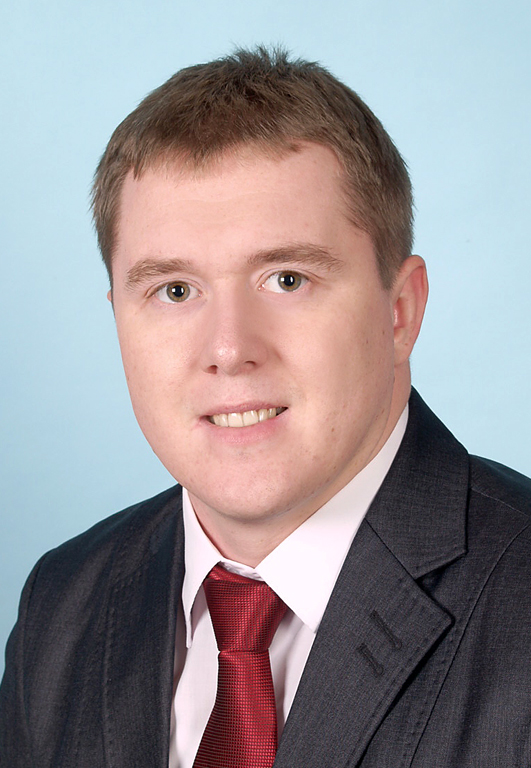
\includegraphics[height=6.5cm,width=4.5cm]{img/foto.jpg}
    \end{minipage}
    &
    \begin{minipage}{12cm}
    \begin{flushleft}
    \par\noindent\vspace{1\baselineskip}
    \begin{tabular}[h]{l l}
    {\normalsize\it Specjalność:} & Informatyka -- \\
    & Inżynieria Systemów Informatycznych
    \end{tabular}
    \par\noindent\vspace{1\baselineskip}
    \begin{tabular}[h]{l l}
    {\normalsize\it Data urodzenia:} & {\normalsize 16 sierpnia 1990~r.}
    \end{tabular}
    \par\noindent\vspace{1\baselineskip}
    \begin{tabular}[h]{l l}
    {\normalsize\it Data rozpoczęcia studiów:} & {\normalsize 22 lutego 2010 r.}
    \end{tabular}
    \par\noindent\vspace{1\baselineskip}
    \end{flushleft}
    \end{minipage}
    \end{tabular}
    \vspace*{1\baselineskip}
    \begin{center}
	{\large\bfseries Życiorys}\par\bigskip
    \end{center}

    \indent
Nazywam się Konrad Miziński. Urodziłem się 16 sierpnia 1990 roku w Grójcu. W 2009 roku ukończyłem XXI Liceum Ogólnokształcące im. H. Kołłątaja w Warszawie. Następnie rozpocząłem studia na Wydziale Elektroniki i Technik Informacyjnych Politechniki Warszawskiej. Zawodowo, od czerwca 2012 roku, związany jestem z Infovide-Matrix S.A. W 2013 roku uzyskałem certyfikat Oracle Certified Associate, Java SE 7 Programmer.
    \par
    \vspace{2\baselineskip}
    \hfill\parbox{15em}{{\small\dotfill}\\[-.3ex]
    \centerline{\footnotesize podpis studenta}}\par
    \vspace{3\baselineskip}
    \begin{center}
 	{\large\bfseries Egzamin dyplomowy} \par\bigskip\bigskip
    \end{center}
    \par\noindent\vspace{1.5\baselineskip}
    Złożył egzamin dyplomowy w dn. \dotfill
    \par\noindent\vspace{1.5\baselineskip}
    Z wynikiem \dotfill
    \par\noindent\vspace{1.5\baselineskip}
    Ogólny wynik studiów \dotfill
    \par\noindent\vspace{1.5\baselineskip}
    Dodatkowe wnioski i uwagi Komisji \dotfill
    \par\noindent\vspace{1.5\baselineskip}
    \dotfill

    % Streszczenie
    \newpage\thispagestyle{empty}
    \vspace*{2\baselineskip} 
    \begin{center}
	{\large\bfseries Streszczenie}\par\bigskip
    \end{center}

    {\itshape
Celem pracy było stworzenie prototypu aplikacji wspomagającej obsługę umów cywilno-prawnych. Kolejne jej rozdziały opisują proces projektowania takiej aplikacji. Sam cel pracy oraz jego motywacja zostały opisane w rozdziale pierwszym. Kolejny rozdział zawiera szczegółowy opis dziedziny oraz przegląd rozwiązań dostępnych na rynku. Zawiera on informacje o rodzajach umów, ich opodatkowaniu i oskładkowaniu. Rozdział trzeci zawiera opis technologii służących do tworzenia aplikacji w architekturze trójwarstwowej. Szczególny nacisk kładzie na te, które zostały wykorzystane w projektowanym systemie. Kolejny rozdział zawiera analizę wymagań projektowych. Rozdział piąty opisuje model danych w postaci diagramów związków encji oraz schematu tabel. W kolejnym rozdziale opisane zostały szczegóły implementacyjne systemu. Całość zakończona jest krótkim podsumowaniem. 

  }
    \vspace*{1\baselineskip}

    \noindent{\bf Słowa kluczowe}: {\itshape umowa cywilno-prawna, umowa zlecenia, umowa o dzieło, architektura trójwarstwowa, aplikacja internetowa}
    \par
    \vspace{4\baselineskip}
    \begin{center}
	{\large\bfseries Abstract}\par\bigskip
    \end{center}
    \noindent{\bf Title}: {\itshape System supporting the service of civil law contracts - three-tier architecture application}\par
    \vspace*{1\baselineskip}
    {\itshape
    	The aim of this work was to create a prototype application supporting service of civil law contracts. Individual chapters describe: civil law contracts, technology overview, requirements analysis, data model and implementation.}
    \vspace*{1\baselineskip}
		
    \noindent{\bf Key words}: {\itshape civil law contract, three-tier architecture, web application}

\end{titlepage}
\end{document}


\tableofcontents
% \addcontentsline{toc}{chapter}{{Przedmowa1}{vii}}{vii}

% \chapter*{Spis tablic, rysunków i~wydruków}
% \listoftables
% \listoffigures
% \lstlistoflistings

%\setlength{\baselineskip}{7mm}
\newpage
\pagenumbering{arabic}
\setcounter{page}{1}


\chapter{Wprowadzenie}

\section[Motywacja][Motywacja]{Motywacja}
W okresie kryzysu gospodarczego pracy coraz częstsze stają się alternatywne formy zatrudnienia takie jak umowy cywilno-prawne. Służą one nie tylko do redukowania kosztów pracy, ale mają zastosowanie wszędzie tam gdzie pracodawcy nie chcą nawiązywać trwałego stosunku pracy na podstawie bezterminowej umowy o pracę. Doskonale sprawdzają się w przypadku zlecania małych zadań wykonywanych również dla własnego pracodawcy. Pojawiają się także na Politechnice Warszawskiej. Wraz z narastająca ich liczbą zaistniała potrzeba automatyzacji procesu obsługi takich umów.

\section[Tytuł w paginie][Tytuł w spisie treści]{Cel pracy}
Celem pracy jest zaprojektowanie oraz implementacja prototypu aplikacji wspomagającej korzystanie z umów cywilno-prawnych, przeznaczonej dla instytucji typu uczelnia. Aplikacja powinna oferować funkcjonalności związane z obsługą umów i zatrudnianych na nie pracowników oraz uwzględniać strukturę organizacji dla której jest przeznaczona. Kolejnym założeniem projektowym jest wykorzystanie architektury trójwarstwowej, tzn podziału aplikacji na warstwę prezentacji(realizowanej przez przeglądarkę internetową), warstwę aplikacji i warstwę źródła danych.

\chapter{Umowy cywilno prawne}
Rozdział ten opisuje umowy cywilno-prawno z prawnego punktu widzenia. Na początku określa samo pojęcie umowy, następnie zwraca uwagę na szczegóły związane z ich opodatkowaniem i oskładkowaniem. Prezentuje przykłady osób zatrudnianych na umowy cywilno-prawne opisując szczegółowo jakie składki powinny być od nich odprowadzane. Na koniec dokonuje krótkiego przeglądu dostępnych na rynku programów wspomagających obsługę umów cywilno-prawnych

\section[Umowa cywilno-prawna][Umowa cywilno-prawna]{Umowa cywilno-prawna}
Słownik języka polskiego \cite{TODO} definije umowę jako pisemne lub ustne porozumienie stron, mające na celu ustalenie wzajemnych praw i obowiązków. W polskim prawie jest najważniejszą postacią czynności prawnych. Podstawowe regulacje dotyczące umów zostały umieszczone w części ogólnej Kodeksu Cywilnego(art. 66-72) \cite{TODO}. Kodeks cywilny reguluje wiele rodzajów umów(m.in. sprzedarzy, pożyczki, ubezpieczenia etc...), z których dwie mogą posłużyć jako alternatywne (w stosunku do umowy o pracę) formy zatrudnienienia. Są to umowa zlecenia oraz umowa o dzieło.

\subsection[Umowa zlecenia][Umowa zlecenia]{Umowa zlecenia}
Umowa zlecenia została uregulowana przez Kodeks Cywilny w art. 734-751 \cite{TODO}. Przez umowę zlecenia zleceniobiorca zobowiązuje się do dokonania określonej czynności prawnej dla zleceniodawcy. Umowa zlecenia bywa nazywana jako umowa starannego działania. Oznacza to, że wynagrodzenie z tytułu umowy zlecenia przysługuje już za samą pracę wykonywana na rzecz zleceniodawcy, nie zaś za jej rezultat.

\subsection[Umowa o dzieło][Umowa o dzieło]{Umowa o dzieło}
Umowa o dzieło została określona przez Kodeks Cywilny w art 627-646\cite{TODO}. Najważniejszym jej elementem jest tzw. Dzieło - rezultat umowy. Poprzez zawarcie strony zobowiązują się z jednej stony do wykoniania dzieła oraz z drugiej stony do wypłaty wynagrodzenia za jego wykonanie. Dziełem może być byt materialny(np. remont budynku), niematerialny(utwór muzyczny, program komputerowy) lub doprowadzenie do ustalonego stanu(np. przeszkolenie pracownika). W momencie zawierania umowy powinno być ono precyzyjnie określone. W przeciwieństwie do umowy zlecenia umowa o dzieło nazywana jest umową rezultatu oznacza to, że wynagrodzenie z tytułu umowy o dzieło przysługuje za osiągnięcie konkretnego efektu a nie za samą pracę(jak w przypadku umowy zlecenia).

\section[Strony umowy][Strony umowy]{Strony umowy}
Wyróżniamy następujące stony stusunku prawnego zaistniałego na podstawie umówy cywilno-prawnej:
\begin{itemize}
	\item Zleceniodawcę(dającego zlecenie) - stronę zlecającą wykonanie okręślonych czynności,
	\item Zleceniobiorcę(przymującego zlecenie) - stronę zobowiązującą się do wykonania tych czynności
\end{itemize}
w przypadku umowy zlecenia, oraz
\begin{itemize}
	\item Zamawiąjącego - stronę zlecającą wykonanie dzieła i zobowiązującą się do wypłaty wyngrodzenia;
	\item Wykonawcę - stronę zobowiązującą się do wykonania dzieła
\end{itemize}
w przypadku umowy o dzieło.

Stronami umowy mogą być zarówno osoby fizyczne jak i osoby prawne.

\section[Forma umowy][Forma umowy]{Forma umowy}
Umowa może zostać zawarta w dowolnej formie, a zatem możemy ograniczyć się do formy ustnej. Zawarcie umowy w formie pisemnej wymaga dla swojej ważności podpisów obu stron. Podpis powinien być podpisem własnoręcznym, dopuszczalny jest też podpis elektroniczny.

\subsection[Elementy obowiązkowe na umowie][Elementy obowiązkowe na umowie]{Elementy obowiązkowe na umowie}
Umowa powinna określać:
\begin{itemize}
\item rodzaj zawartej umowy, która powinna wynikać z nazwy i treści,
\item strony umowy,
\item przedmiot umowy,
\item datę rozpoczęcia jak i zakończenia wykonywania umowy,
\item informację czy umowa ma być wykonywana u zleceniodawcy badź zamawiającego,
\item zasady ustalania wynagrodzenia.
\end{itemize}

\section[Wypowiedzenie umowy][Wypowiedzenie umowy]{Wypowiedzenie umowy}
Umowa może być w każdym czasie jednostronnie rozwiązana przez którąkolwiek ze stron. W przypadku umowy odpłatnej zlecający jest ma obowiązek uiścić wykonawcy badź zleceniobiorcy część wynagrodzenia odpowiadającą jego dotychczasowym czynnościom, a jeżeli wypowiedzenie nastąpiło bez ważnego powodu, powinien także naprawić wynikłą stąd szkodę. W przypadku gdy umowę wypowiada przyjmujący zlecenie bądź wykonawca dzieło jest on odpowiedzialny za szkodę jaką poniósł zleceniodawca badź zamawiający dzieło.

\section[Powierzenie wykonywania umowy osobie trzeciej][Powierzenie wykonywania umowy osobie trzeciej]{Powierzenie wykonywania umowy osobie trzeciej}
Jeśli w umowie nie zostało zapisane, że musi być wykonana osobiście możliwe jest powierzenie jej wykonania osibie trzeciej.

\section[Wynagrodzenie][Wynagrodzenie]{Wynagrodzenie}
Umowa zlecenia może być zarówno umową odpłatną jak i nieodpłatną, w zależności od ustaleń stron, przy czym jeśli zlecenie ma być nieodpłatne, informacja o tym musi znaleźć się w umowie. W przeciwnym razie uznaje się, że zlecenie jest wykonywane odpłatnie. Umowa o dzieło jest zawsze umową odpłatną. Umowa może jednak nie określać dokładnie wysokości wynagrodzenia. Zamiast tego może zawierać podstawy służące do jego ustalenia. Jeśli i tych brak to kwota wynagrodzenia powinna być adekwatna do czasu poświęconego na daną pracę.

Zapłata wynagrodzenia następuje z reguły już po wykonaniu umowy. Strony mogą jednak dowolnie ustalić termin płatności wynagrodzenia, jak i sposób zapłaty(jednorazowy, lub ratalny). Nie ma obowiązku stosowania zasady stosowania comiesięcznej wypłaty przy umowach zawieranych na dłuższy czas. Można pozostać zarówno przy zasadzie rozliczenia po zakończeniu umowy jak i wprowadzić rozliczenia w krótszych okresach.

\subsection[Rachunek do umowy][Rachunek do umowy]{Rachunek do umowy}
Kwestie rachunków reguluje rozdiał 12 ordynacji podatkowej\cite{TODO}. W ogólnym przypadku nie ma obowiązku wystawiania rachunku do umowy. Obowiązek taki występuję wtedy gdy zostało to zastrzeżone w umowie lub na życzenie zamawiającego. W takim przypadku rachunek powinien zostać wystawiony w terminie 7 dni od daty wynikającej z umowy lub jego zażądania przez zamawiającego.Rachunek powinien zawierać:
\begin{itemize}
\item numer rachunku - ustawodawca nakłada na wystawiającego obowiązek numerowania rachunków,
\item datę wystawienia,
\item strony umowy,
\item przedmiot umowy,
\item cęnę (jednostkową i ogólną - jeśli przedmiot umowy został wykonany kilka razy).
\end{itemize}

\subsection[Protokół odbioru dzieła lub zlecenia][Protokół odbioru dzieła lub zlecenia]{Protokół odbioru dzieła lub zlecenia}
Podobnie jak w przypadku rachunków kodeks cywilny nie nakłada obowiązku sporządzania takiego protokołu. Należy go jednak sporządzić jeśli zostało to zaznaczone w umowie. Protokół taki może stanowić podstawę do wypłaty wynagrodzenia badź wystawienia rachunku. Pozwala też jednoznacznie stwierdzić,że(i kiedy) nastąpiło odebranie dzieła lub zlecenia.

\section[Opodatkowanie][Opodatkowanie]{Opodatkowanie}
Zasady opodatkowania umów cywilno-prawnych definiuje ustawa o podatku dochodowym od osób fizycznych\cite{TODO}. W sytuacji, gdy wynagrodzenie z tytułu umowy nie przekracza 200 złotych brutto, przychód podlega opodatkowaniu zryczałtowanym podatkiem dochodowym w wysokości 18\%, bez uwzględniania składek na ZUS i kosztów uzyskania przychodu.
W przypadku wynagrodzenia powyżej 200 złotych brutto, przychód podlega opodatkowaniu na zasadach ogólnych z uwzględnieniem składek ZUS oraz kosztów uzyskania przychodu.

\subsection[Koszty uzyskania przychodu][Koszty uzyskania przychodu]{Koszty uzyskania przychodu}
W myśl art. 22 ustawy o podatku dochodowym od osób fizycznych\cite{TODO} kosztami uzyskania przychodów są koszty poniesione w celu osiągnięcia przychodów lub zachowania albo zabezpieczenia źródła przychodów. Odlicza się je od wynagrodzenia(po uprzednim odliczeniu składek na ZUS) i dopiero od tak obliczonej kwoty odprowadza się podatek. W większości umów koszty uzyskania przychodu wynoszą 20\% kwoty przychodu netto natomiast w przypadku umów, które wiążą się z przeniesieniem praw autorskich twórców i artystów, koszty uzyskania przychodu wynoszą 50\%. W szczególnych przypadkach koszty te mogą zostać podwyższone jadnak podatnik musi wtedy udowodnić, że poniesione przez niego koszty są faktycznie wyższe niż zapisane w ustawie.

\subsection[Ograniczenia w stosowaniu podwyższonych kosztów uzyskania przychodu][Ograniczenia w stosowaniu podwyższonych kosztów uzyskania przychodu]{Ograniczenia w stosowaniu podwyższonych kosztów uzyskania przychodu}
Od 1 stycznia 2013 roku wprowadzono ograniczenie stosowania 50-procentowych kosztów uzyskania przychodu. Zakłada ono, że  w przypadkach, o których mowa w \ref{prawaAutorskie} roczne koszty uzyskania przychodu nie mogą przekroczyć połowy górnej granicy pierwszego przediału skali podatkowej(w chwili pisania pracy wynosiła ona 85 528 zł).

\section[Prawa autorskie][Prawa autorskie]{Prawa autorskie}
\label{prawaAutorskie}
Przypadki, w których możemy kożystać z praw autorkich(a co za tym idzie z podwyższonych kosztów uzyskania przychodu) definiuje art. 22 ust.9 pkt 1-3 ustawy o podatku dochodowym od osób fizycznych\cite{TODO}, są to
\begin{itemize}
	\item  zapłata twórcy za przeniesienie prawa własności wynalazku, topografii układu scalonego, wzoru użytkowego, wzoru przemysłowego, znaku towarowego lub wzoru zdobniczego,
	\item opłata licencyjna za przeniesienie prawa stosowania wynalazku, topografii układu scalonego, wzoru użytkowego, wzoru przemysłowego, znaku towarowego lub wzoru zdobniczego, otrzymanej w pierwszym roku trwania licencji od pierwszej jednostki, z którą zawarto umowę licencyjną,
	\item korzystanie przez twórców z praw autorskich i artystów wykonawców z praw pokrewnych, w rozumieniu odrębnych przepisów, lub rozporządzanie przez nich tymi prawami.
\end{itemize}
Typ umowy nie ma w tym przypadku znaczenia. Może to być zarówno umowa zlecenia, umowa o dzieło jak i inna umowa(np. umowa o pracę czy umowa o przeniesienie praw autorskich).

W przypadku omawianych umów cywilno-prawnych umowę o charakterze autorskim należy zawrzeć wtedy gdy przedmiot umowy stanowi przedmiot prawa autorskiego(utwór) w rozumieniu art. 1 ustawy o prawie autorskim i prawach pokrewnych\cite{TODO}. Przeniesienie praw autorskich wymaga pisemnej formy umowy.

\section[Ubezpieczenia społeczne i ubezpieczenie zdrowotne][Ubezpieczenia społeczne i ubezpieczenie zdrowotne]{Ubezpieczenia społeczne i ubezpieczenie zdrowotne}
Od umów cywilno-prawnych mogą być pobierane składki na następujące ubezpieczenia:
\begin{itemize}
	\item ubezpieczenia społeczne:
	\begin{itemize}
		%TODO mozesz dodac opisy poszczególnych ubezpieczeneń
		\item ubezpieczenia emerytalne,
		\item ubezpieczenia rentowe,
		\item ubezpiecznie chorobowe,
		\item ubezpiecznie wypadkowe,
	\end{itemize}
	\item ubezpieczenie zdrowotne.
\end{itemize}
Zasady odporwadzania skaładek na ubezpieczenie społeczne od umów cywilno-prawnych definiuje rozdział 2 ustawy o systemie ubezpieczeń społecznych\cite{TODO} zaś na ubezbieczenie zdrowotne dział IV ustawy o świadczeniach opieki zdrowotnej finansowanych ze środków publicznych\cite{TODO}.

\subsection[Ubezpieczenie emerytalne i ubezpieczenie rentowe][Ubezpieczenie emerytalne i ubezpieczenie rentowe]{Ubezpieczenie emerytalne i ubezpieczenie rentowe}
Obowiązek odprowadzania składek na ubezpieczenia emerytalne i rentowe uzależniony jest od wielu czynników m. in. tego czy osoba zatrudniona na umowę cywilno-prawną ma już podpisaną umowę o pracę, przychodu z tytułu tej umowy czy pracowdawcy, z którym umowa została zawarta. Zostanie on wyjaśniony na przykładach w dalszej części rozdziału w punkcie\ref{przykladyOsob}.

\subsection[Ubezpiecznie chorobowe][Ubezpiecznie chorobowe]{Ubezpiecznie chorobowe}
Odporwadzanie skałdek na ubezpieczenie chorobowe jest możliwe tylko wtedy gdy zatrudniony na umowę cywilno-prawną podlega \textbf{obowiązkowym} ubezpieczeniom emertytalnym i rentowym. W zależności od sytuacji może być ono obowiązkowe lub dobrowolne.

\subsection[Ubezpiecznie wypadkowe][Ubezpiecznie wypadkowe]{Ubezpiecznie wypadkowe}
Zatrudniony na umowę cywilno prawną podlega obowiązkowemu ubezpieczeniu wypadkowemu zawsze wtedy gdy podlega ubezpieczeniom emerytlanemu i rentowemu(niezależnie od tego czy podlega tym ubezpieczeniom obowiązkowo czy dobrowolnie).

\subsection[Ubezpieczenie zdrowotne][Ubezpieczenie zdrowotne]{Ubezpieczenie zdrowotne}
Zasady odprowadzania składek na ubezpieczenie zdrowotne są zdefiniowane w innej ustawie niż zasady odprowadzania składek na ubezpieczenia społeczne. Dla uproszczenia można przyjąć zasadę że obowiązek odprowadzania składek na ubezpieczenie zdrowotne ma miejsce wszędzie tam gdzie występuje obowiązek lub możliwość(ubezpieczenie dobrowolne) odpowadzania składek na ubezpieczenia emerytalne i rentowe. Ustawodawca nie przewidział możliwości dobrolnego odprowadzania składek na ubezpieczenie zdrowotne.

\section[Przykłady osób zatrudnionych na umowach cywilno-prawnych][Przykłady osób zatrudnionych na umowach cywilno-prawnych]{Przykłady osób zatrudnionych na umowach cywilno-prawnych}
\label{przykladyOsob}

\subsection[Pracownik zatrudniony na umowę o pracę][Pracownik zatrudniony na umowę o pracę]{Pracownik zatrudniony na umowę o pracę}
\label{umowaOPrace}
Jest to przypadek najbardziej złożony. Można go podzielić na 2 mniejsze podprzypadki:

\subsubsection{Umowa cywilno-prawna zawarta z własnym pracodawcą lub wykonywana na rzecz własnego pracowawcy}
W tym przypadku pracodawca ma obowiązek odprowadzać wszytkie ubezpieczenia(emerytalne, rentowe, chorobowe, wypadkowe i zdrowotne) za swojego pracownika.

\subsubsection{Umowa cywilno-prawna nie zawarta z własnym pracodawcą i nie wykonywana na jego rzecz}
W tym przypadku zatrudniony na umowę o dzieło nie podlega(ani dobrowolnie, ani obowiązkowo) żednemu z ubezpieczeń społecznych ani ubezpieczeniu zdrowotnemu. 

W przypadku umowy zlecenia pod uwagę brany jest pod uwagę przychód z tytułu umowy o pracę. Jeśli jest on niższy od minimalnego wynagrodzenia za pracę(lub jego 80\% w przypadku osób zatrudnionych krócej niż 1 rok) to zleceniobiorca podlega obowiązkowym ubezpieczeniom emerytalnemu, rentowemu i wypadkowemu, może podlegać dobrowolnemu ubezpieczeniu chorobowemu, podlega obowiązkowemu ubezpieczeniu zdrowotnemu. W przeciwnym wypadku może dobrolnie podlegać ubezpieczeniom emerytalnemu i rentowemu(co pociąga za sobą obąwiązkowe podleganie ubezpieczeniu wypadkowemu), nie może podlegać ubezpieczeniu chorobowemu, podlega obowiązkowemu ubezpieczeniu. Od 1 stycznia 2014 roku minimalne wynagrodzenie za pracę(tzw. płaca minimalna) wynosi 1680 zł brutto.

\subsection[Uczeń lub student do 26 roku życia][Uczeń lub student do 26 roku życia]{Uczeń lub student do 26 roku życia}
Od umów zawartych ze studentami oraz uczniami szkół ponadgimnazjalnych nie odprowadza się składek na ubezpieczenia społeczne ani na ubezpiecznie zdrowotne. Zwolnienie to rozciąga się na okres do ukończenia przez nich 26 roku życia. Osoby kończące szkołe są traktowanie do 31 sierpnia(do końca wakacji)  tak jakby ciągle były uczniami danej szkoły(lub do 30 września w przypadku przyjęcia na studia wyższe). Datą ukończenia studiów jest data złożenia egzaminu dyplomowego. Utrata statusu studenta następuje także w przypadku skreślenia z listy studentów.

\subsection[Osoba niemająca innego tytułu ubezpieczenia niż umowa cywilno-prawna][Osoba niemająca innego tytułu ubezpieczenia niż umowa cywilno-prawna]{Osoba niemająca innego tytułu ubezpieczenia niż umowa cywilno-prawna}
\label{inni}
W tym przypadku występuje obowiązek odprowadzania składek na ubezpieczenia emerytalne, rentowe, wypadkowe oraz ubezpieczenie zdrowotne od umowy zlecenia, oraz możliwość do dobowolnego przystąpiania do ubezpieczenia chorobowego. Jeśli jednak zleceniobiorca podpisze równolegle kilka umów zleceń to znika obowiązek odprowadzania składek na ubezpieczenia emerytalne i rentowe od kolejnych umów(stają się one dobrowolne), nie ma też możliwości podlegeania ubezpieczeniu chorobowemu, pozostaje jednak obowiązek podlegania ubezpieczeniu zdrowotnwemu(musi być ono odprowadzane od każdej umowy), ubezpieczenie wypadkowe jest uzależnione od ubezpieczeń emyratalnego i chorobowego.

W przypadku umowy o dzieło wykonawca nie podlega ubezpieczeniom społecznym ani ubezpieczeniu zdrowotnemu.

\subsection[Emeryt lub rencista][Emeryt lub rencista]{Emeryt lub rencista}
Emerytów i rencistów obowiązują w ogólności takie same zasady jak osoby nie mające innego tytułu ubezpieczenia(patrz \ref{inni}).
Wyjątkiem jest sytuacja, w której emeryt lub recnicta jest zatrudniony na umowę o pracę(porównaj \ref{umowaOPrace}). Można tu również wyróżnić 2 przypadki:

\subsubsection{Umowa cywilno-prawna zawarta przez emeryta lub rencistę z własnym pracodawcą lub wykonywana na rzecz własnego pracowawcy}
W tym przypadku pracodawca(tak jak w przypadku zwykłego pracownika)ma obowiązek odprowadzać wszytkie ubezpieczenia(emerytalne, rentowe, chorobowe, wypadkowe i zdrowotne).

\subsubsection{Umowa cywilno-prawna nie zawarta przez emeryta lub rencistę z własnym pracodawcą i nie wykonywana na jego rzecz}
W przypadku umowy o dzieło emeryt lub rencista traktowany jest jak zwykły pracownik i nie podlega ubezpieczeniom społęcznym ani ubezpieczeniu zdrowotnemu. Różnica występuje natomiast w przypadku umowy o dzieło. Nie zależnie od przychodu z tytułu umowy o pracę zleceniobiorca jest traktowany tak jakby jego wynagrodzenie ze stosunku pracy było większe bądź równe płacy minimalnej. Może on wtedy podlegać dobrowolnie ubezpieczeniom emerytalnemu i rentowemu(a co za tym idzie również wypadkowemu), nie może podlegać ubezpieczeniu chorobowemu oraz podlega obowiązkowemu ubezpieczeniu zdrowotnemu.

\subsection[Osoba pobierająca zasiłek macieżyński][Osoba pobierająca zasiłek macieżyński]{Osoba pobierająca zasiłek macieżyński}
W przypadku umów zleceń osoba pobierająca zasiłek macieżyński może dobrolnie podlegać ubezpieczeniom emerytalnemu i rentowemu(co pociąga za sobą obąwiązkowe podleganie ubezpieczeniu wypadkowemu), nie może podlegać ubezpieczeniu chorobowemu, podlega obowiązkowemu ubezpieczeniu zdrowotnemu. W przypadku umów o dzieło osoba taka nie podlega ubezpieczeniom społecznym ani ubezpieczeniu zdrowotnemu.

\subsection[Osoba przybywająca na urlopie wychowawczym][Osoba przybywająca na urlopie wychowawczym]{Osoba przybywająca na urlopie wychowawczym}
Osoba przybywająca na urlopie wychowawczym z punku widzenia ubezpieczeń społecznych i ubezpieczenia zdrowotnego taktowanana jset tak osoba niemająca innego tytułu ubezpieczenia niż umowa cywilno-prawna(partrz \ref{inni}).

\subsection[Osoba prowadząca działalność gosprodarczą][Osoba prowadząca działalność gosprodarczą]{Osoba prowadząca działalność gosprodarczą}
Jeśli umowa cywilno-prawna jest wykonywana w ramach prowadzonej działalności gospodarczej to nie podalega ona bezpieczeniom społecznym ani ubezpieczeniu zdrowotnemu. W przeciwnym wypadku osoba zatrudniona na taką umowę powinna być traktowana jak osoba zatrudniona na umowę o pracę u pracodawcy innego niż zleceniodawca badź zamawiający dzieło(patrz \ref{umowaOPrace}).

\section{Składki na Fundusz Gwarantowanych Świadczeń Pracowniczych i Fundusz Pracy}
Obowiązek odporwadzania składek na Fundusz Gwarantowanych Świadczeń Pracowniczych i Fundusz Pracy regulują odpowiedznio ustawa o ochronie roszczeń pracowniczych w razie niewypłacalności pracodawcy\cite{TODO} i ustawa o promocji zatrudnienia i instytucjach rynku pracy. Obowiązek taki występuje gdy zatrudniony na umowę cywilno-prawną:
\begin{itemize}
	\item podlega obowiązkowym ubezpieczeniom emerytalnemu i rentowym oraz
	\item uzyskuje z tytułu umowy przychód w wysokości co najmniej minimalnego wynagrodzenia za prace
\end{itemize}
Sładek na Fundusz Gwarantowanych Świadczeń Pracowniczych i Fundusz Pracy nie odprowadza się po ukończeniu 55 lat(w przypadku kobiet) lub 60 lat(w przypadku mężczyzn).

\section[Umowy cywilno-prawne a prawo pracy][Umowy cywilno-prawne a prawo pracy]{Umowy cywilno-prawne a prawo pracy}
W przypadku umów cywilno-prawnych nie zachodzi stosunek pracy, nie ma więc zastosowania prawo pracy(w sczególności kodeks pracy). Zatrudniony na taką umowę nie ma więc prawa do płatnych ulropów. Nie ma również możliwości kożystania ze zwolnienia lekarskiego.

\section[Systemy wspomagające obsługę umów cywilno-prawnych][Systemy wspomagające obsługę umów cywilno-prawnych]{Systemy wspomagające obsługę umów cywilno-prawnych}

\subsection[Kalkulatory wynagrodzeń][Kalkulatory wynagrodzeń]{Kalkulatory wynagrodzeń}
Najprostrzym przykładem aplikacji wspomagającej obsługę umów cywilno-prawnych są kalkulatory wynagrodzeń. Pozwalają one na oblicznie wynagrodzenie netto na podstawie podanego wynagrodzenia brutto, oraz informacji o koszcie uzyskania przychodu oraz składkach odprowazanych na ubezpieczenia społeczne i ubezpieczenie zdrowotne. Na rysunku \ref{kalkulator} przedstawiono przykładowy kalkulator dostępny w internecie na strone www.kalkulatory.gofin.pl.

\begin{figure}[tdh]
    \begin{center}
	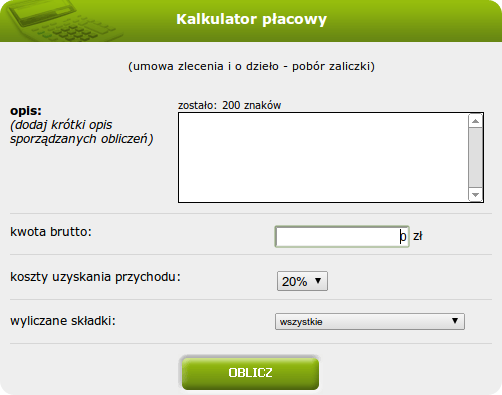
\includegraphics[scale=.6]{img/kalkulator.png}
	\caption{Kalkulator wybagrodzeń z tytułu umów cywilno-prawnych}
	\label{kalkulator}
    \end{center}
\end{figure}

\subsection[SystemUmów.pl][SystemUmów.pl]{SystemUmów.pl}
SystemUmów.pl jest dedykowaną aplikacją internetową frmy KotKla do obsługi umów zleceń oraz o dzieło. Zapewnia ona przede wszystkim:
\begin{itemize}
	\item dodawanie oraz archiwizację umów,
	\item szablony umów(bogata baza dostępnych szablonów oraz możliwość definiowania własnych),
	\item dodawanie pracowników oraz przechowywanie ich danych,
	\item ręczne generowanie rachunków na podstawie szablonów(wbudowanych lub zdefiniowanych własnoręcznie),
	\item export umów i rachunków do formatu pdf,
	\item miesięcznie oraz roczne deklaracje PIT i ZUS,
	\item możliwość definiowania danych (takich jak nazwa, adres, NIP czy REGON) własnej firmy.
\end{itemize}

Jest to aplikacja płatna(150 zł za rok badź 3000 zł za licęcję dożywotnią), ale istnieje też jej darmowa wersja. Charkteryzuje się ona następującymi ograniczeniami:
\begin{itemize}
	\item czas trwania licencji ograniczony do 90 dni,
	\item ilość włąsbych szablonów ograniczona do 3,
	\item liczba umów ograniczona do 50.
\end{itemize}
Program pozwala na łatwe realizowanie podstawych funkcji związanych z obsługą umów cywilno prawnych, łatwo jednak zauważyć kilka podstawowych ograniczeń.
\begin{itemize}
	\item możliwość generacji tylko jednego rachunku do każdej umowy - ogranicza to możliwość ratalnej wypłaty wynagrodzenia.
	\item reczna generecja rachunku na podstawie szablonu pozwala wygenerewać rachunek nie adekwatny do umowy(np. rachunek informujący o 50\% koszcie uzyskania przychodu do nieautorskiej umowy.) wymaga też znajomości składek ZUS pracownika przy każdorazoewj generacji.
	\item brak możliwości podziału przedsiębiorstwa na mniejsze jednostki, czy wyodrębniania poszczególnych zadań.
\end{itemize}

Na rysunku \ref{kotkla-systemumow} przedstawiono przykładowy zrzut ekrany z aplikacji SystemUmów.pl

\begin{figure}[tdh]
    \begin{center}
	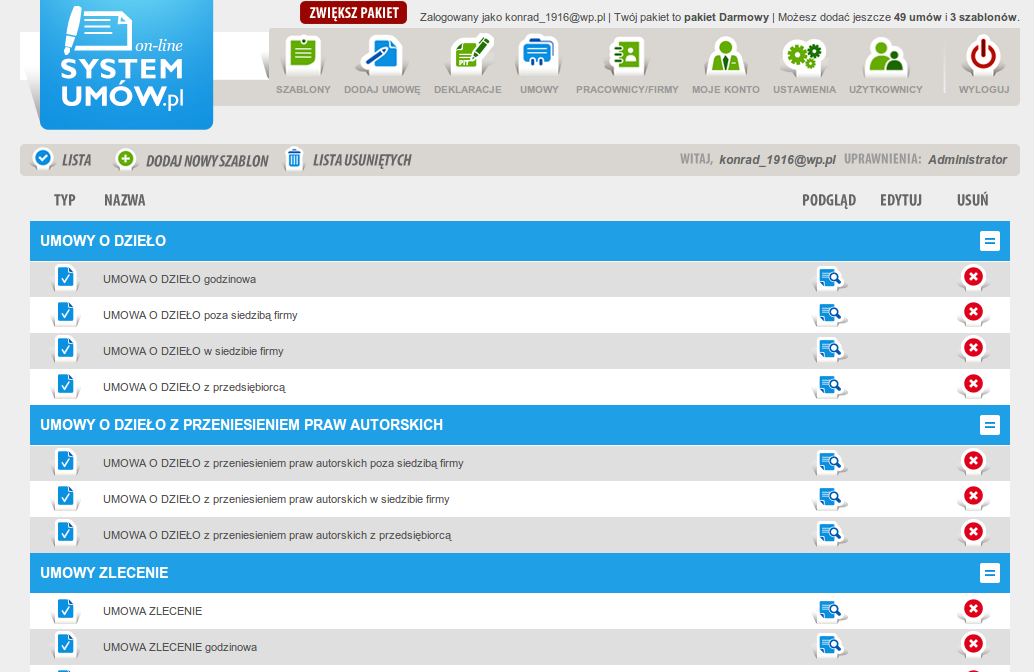
\includegraphics[scale=.4]{img/kotkla-systemumow.png}
	\caption{Lista szablonów umów cywilno-prawnych w aplikacji KotKla-SystemUmów.pl}
	\label{kotkla-systemumow}
    \end{center}
\end{figure}

\subsection[Asystent Rejestr Umów][Asystent Rejestr Umów]{Asystent Rejestr Umów}
Asystent Rejest Umów to program firmy Meteoryt Software. Ma on format aplikacji aplikacji desktopowej korzystającej z bazy danych(lokalnej lub zdalnej). Jest to bardzo zaawansowana aplikacja pozwalająca nie tylko na zarządzanie umowami ale też zaradzanie zadaniami, danynymi kontraktowymi, wspierająca system sprzedarzy czy służąca do fakturowania. Pozwala na obsługę nie tylko umów zleceń czy o dzieło ale też(a raczej przede wszystkim) umów takich jak umowa o pracę czy umowa kupna-sprzedaży. Zepwenia obsługę takich szczegółów jak okres wypowiedzenia czy miejsce prezechowywania oryginału umowy. Pozwala na wysyłanie notyfikacji w formie e-maili bądź smsów. Jest oczywiście aplikacją płatną a jej ceny wachają się w zależności od wersji(najtańszą wersja PRO kosztuje 99zł za rok użytkowania). Na rysunku \ref{asystent-rejestr-umow} przedstawiono przykładowy zrzut ekrany z aplikacji Asystent Rejestr Umów.

\begin{figure}[tdh]
    \begin{center}
	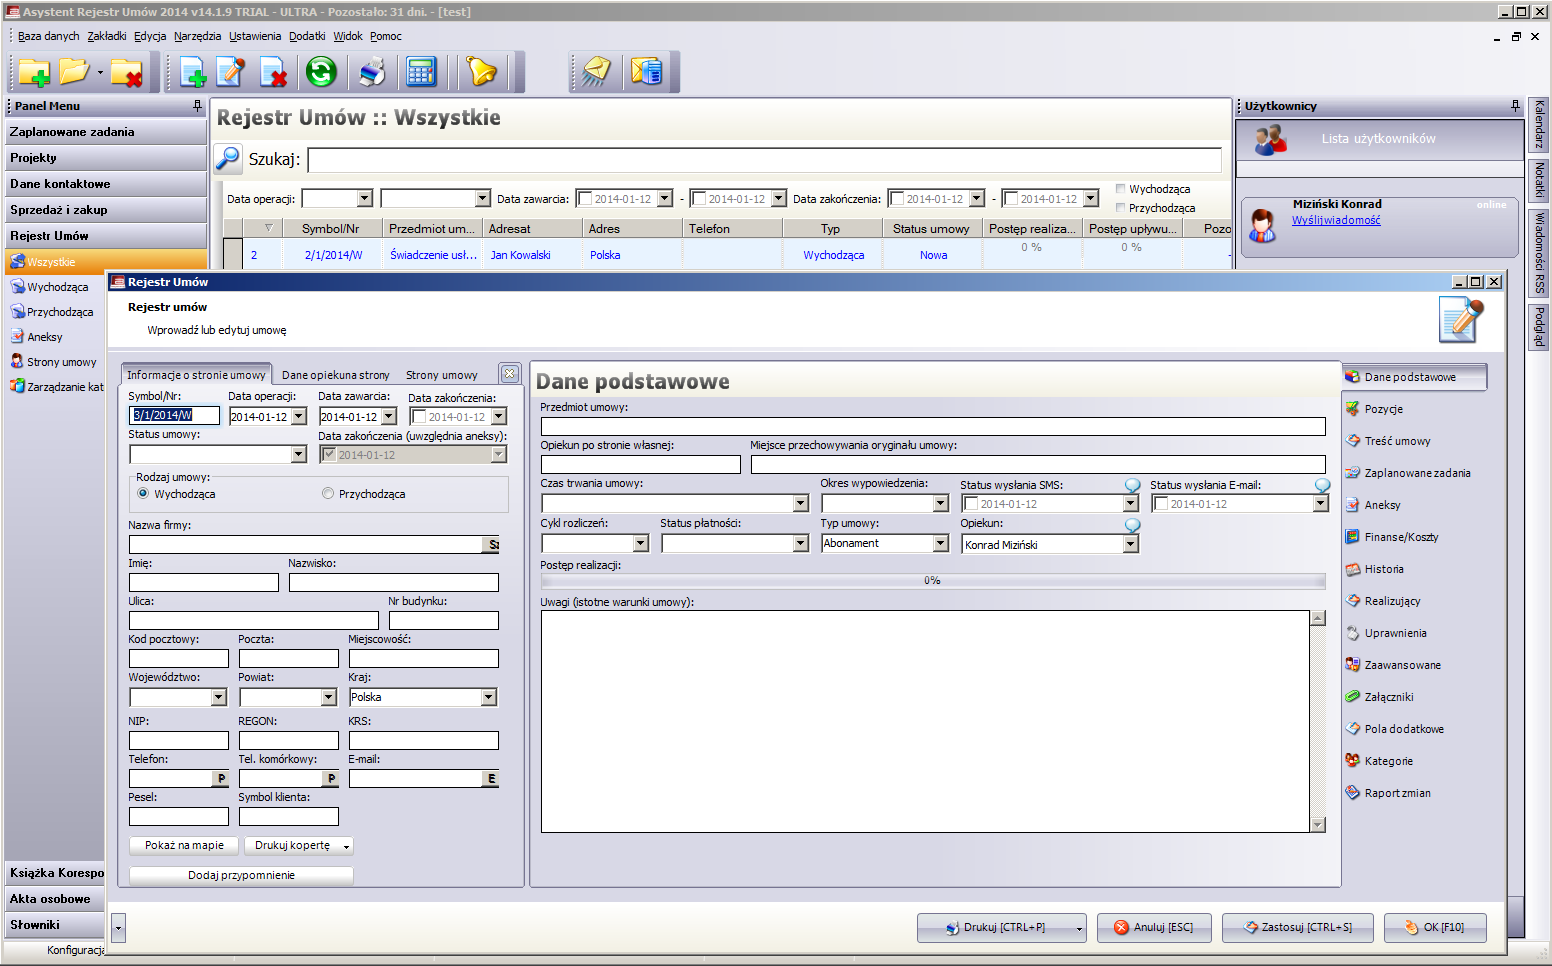
\includegraphics[scale=.6, angle=-90]{img/asystent-rejestr-umow.png}
	\caption{Dodawanie nowej umowy w aplikacji Asystent Rejestr Umów}
	\label{asystent-rejestr-umow}
    \end{center}
\end{figure}

\chapter{Model funkcjonalny}
Poniższy rozdział opisuje proces projektowania aplikacji. Przede wszystkim określa profil odbiorcy sytemu. Prezentuje też wszystkie wymagania jak i założenia poczynione w trakcie ich analizy.

\section[Profil odbiorcy systemu][Profil odbiorcy systemu]{Profil odbiorcy systemu}
Potrzeba stworzenia systemu do obsługi umów cywilno-prawnych powstała na Politechnice Warszawskiej a dokładniej w Ośrodku Kształcenia na Odległość. Początkowa miała ona obsługiwać jedynie umowy zlecenia jednak zdecydowano się ją rozszerzyć również na umowy o dzieło(stąd ogólna nazwa umowy cywilno-prawne). Podczas procesu projektowania starano się jednak aby model był nie tylko dostosowany do specyfiki uczelni ale też jak najbardziej ogólny, tak aby potencjalnym odbiorcą aplikacji mogły być nie tylko uczelnie ale i inne instytucje o podobnej organizacji a nawet małe firmy.

\section[Opis funkcjonalności][Opis funkcjonalności]{Opis funkcjonalności}

\subsection[Pracownicy][Pracownicy]{Pracownicy}
\label{pracownicy}
Aplikacja powinna umożliwiać przechowywanie danych o osobach zatrudnianych na umowach cywilno-prawnych, zwanych dalej potocznie pracownikami(nie są to pracownicy w rozumieniu kodeksu pracy). Podstawowymi operacjami jakie można wykonać na pracowniku jest jego dodanie, modyfikacja oraz usunięcie(ale tylko w przypadku gdy nie ma on podpisanej żadnej umowy). Dodatkowymi funkcjonalnościami są wyszukiwanie pracownika za pomocą imienia i nazwiska oraz możliwość wyświetlenia listy wszystkich pracowników.

Aplikacja będzie gromadzić wszystkie informacje niezbędne jego jednoznacznej identyfikacji, umieszczane na umowach oraz potrzebne w celach podatkowych: nazwisko, imiona(z wyróżnieniem pierwszego imienia), adresy(przy czym należy zwrócić uwagę, że adres wykorzystywany w celach podatkowych może różnić się od adresu korespondencyjnego), datę i miejsce urodzenia, płeć, obywatelstwo(aplikacja powinna udostępniać wybór z listy możliwych państw), numery pesel i NIP, numer dowodu osobistego lub paszportu oraz numer konta. Dodatkowo system powinien przechowywać informację o urzędzie skarbowym(jego nazwę i adres) właściwym dla pracownika. Dane urzędu skarbowego powinny być przechowywane niezależnie od danych pracownika tak aby np. w przypadku zmiany adresu jednego z urzędów nie występowała konieczność ręcznej aktualizacji wszystkich odpowiadających mu pracowników a jedynie pojedyncza modyfikacja danych urzędu skarbowego. Podczas wprowadzania bądź modyfikacji danych pracownika użytkownik powinien mieć możliwość wyboru z listy wcześniej zdefiniowanych urzędów skarbowych lub dodania nowego w przypadku jego braku na liście.

Istotnym elementem danych pracownika jest informacja jakie składki ubezpieczeń będzie musiał odprowadzać od potencjalnie podpisanych umów. Aplikacja powinna przechowywać informacje o jego statusie z punktu widzenia umów cywilno prawnych(opisanym w \ref{przykladyOsob}). Powinna też wspomagać użytkownika w trakcie wyboru statusu - wyświetlać ich szczegółowe opisy oraz powiązane z nimi składki ubezpieczeń. Te informacje powinny być również zawarte w raportach prezentujących dane pracownika. Lista dostępnych statusów jest zdefiniowana w momencie instalacji, nie możliwości jej edycji za pomocą aplikacji.

\subsection[Struktura organizacyjna][Struktura organizacyjna]{Struktura organizacyjna}
Struktura organizacyjna uczelni podobnie jak struktura organizacyjna wielu innych instytucji ma formę drzewa. Dla prawie każdej jednostki organizacyjnej można wskazać jednostkę nadrzędną(Wyjątkiem jest jednostka będąca korzeniem drzewa, z reguły jest to sama organizacja, np konkretna uczelnia). Ponadto jednostki na poszczególnych poziomach drzewa posiadają swoje typy. W przypadku Politechniki Warszawskiej są to np. uczelnia, wydział, instytut i zakład. Nie jest jednak wymogiem aby na jednym poziomie drzewa znajdowały się jednostki tylko jednego typu. Na przykład jednostkami podległymi wydziałowi mogą oprócz instytutów być też dziekanat, czy administracja gmachu. Nie ma też wymogu aby jednostką nadrzędną danej jednostki organizacyjnej był jednostka typu, który jest typem bezpośrednio nadrzędnym do jej typu. Na przykład nie wszystkie zakłady muszą podlegać instytutom, niektóre z nim mogą podlegać bezpośrednio wydziałom. 

Aplikacja powinna udostępniać zestaw typów jednostek oraz definiować który typ jest nadrzędny w stosunku do którego. Dane te powinny być zdefiniowane w momencie instalacji i nie powinno być możliwości ich zmiany z poziomu aplikacji. Program powinien umożliwiać dodawanie nowych jednostek organizacyjnych(nadawanie im nazwy), definiowanie ich typów oraz umieszczanie ich w strukturze organizacji(poprzez nadanie jednostek nadrzędnych). Powinien również umożliwiać ich edycję oraz usuwanie(pod warunkiem, że nie spowoduje to osierocenia innej jednostki organizacyjnej oraz w systemie nie ma zdefiniowanych zadań wykonywanych dla tej jednostki(patrz \ref{zadania})). Aplikacja powinna pilnować struktury drzewa oraz zgodności typów jednostek. Powinna też umożliwić wyszukiwanie jednostki za pomocą jej nazwy, oraz wyświetlania wszystkich jednostek obecnych w systemie.

Atrybutami jednostki oprócz wspominanych wcześniej nazwy, typu i miejsca w strukturze organizacji są jej adres oraz reprezentant, którego zadaniem jest podpisywanie umów w imieniu jednostki. Atrybutami reprezentanta są jego imię i nazwisko jednak ze względu pisemną formę umowy należy przechowywać również formę biernika. Jeden reprezentant może być przypisany do kliku jednostek. Tak jak w przypadku urzędu skarbowego podczas wprowadzania bądź edycji jednostki użytkownik powinien mieć możliwość wyboru reprezentanta z listy już wcześniej wprowadzonych lub dodania nowego.

W trakcie analizy podjęto decyzję, że pracownicy nie będą w żaden sposób połączeni z jedną konkretną jednostką(nawet jeśli są w niej na stałe zatrudnieni).

\subsection[Zadania][Zadania]{Zadania}
\label{zadania}
W ramach jednostek organizacyjnych wykonywane są zadania. To na wykonywanie poszczególnych zadań, bądź ich części zatrudnia się pracowników na umowy cywilno-prawne. Podstawowym atrybutem zadania jest jego nazwa. Zadanie może też posiadać swój opis, budżet, datę rozpoczęcia oraz datę zakończenia. O ile opis pełni charakter jedynie informacyjny, to w przypadku pozostałych atrybutów aplikacja powinna sprawdzać czy umowy podpisywane na wykonanie tego zadanie mieszczą się w zdefiniowanych ramach czasowych(data rozpoczęcia i data zakończenia) oraz czy sumaryczna wartość umów nie przekracza budżetu zdefiniowanego dla danego zadania. Dodatkowo istnieje możliwość oznaczenia zadania jako rozliczone skutkująca tym, że nie będzie można podpisywać już żadnych umów na wykonanie tego zadania. 

Podczas analizy ustalono, że powinna istnieć możliwość podziału zadań na mniejsze grupy w ramach jednostki organizacyjnej. Wprowadzono więc kolejny atrybut zadania jakim jest jego typ(definiowany w ramach jednostki). 

Użytkownik powinien posiadać możliwość dodawania i edycji zarówno zadań jak i ich typów. Usuwanie typów zadań możliwe jest tylko wtedy gdy nie ma żadnego zadania danego typu. Analogicznie usunąć zadanie można tylko wtedy gdy w systemie nie ma żadnych powiązanym z nim umów. Dodatkowo system powinien umożliwiać wyszukiwanie zadań po nazwie oraz ich typie, oraz wyświetlanie wszystkich zadań powiązanych z daną jednostką organizacyjną oraz jednostkami jej podległymi. Analogicznie użytkownik powinien mieć możliwość wyszukiwania typów zadań po ich nazwach oraz możliwość wyświetlania wszystkich typów zadań właściwych dla danej jednostki.

\subsection[Umowy][Umowy]{Umowy}
Najważniejszym obiektem występującym w systemie jest umowa. Podstawowymi atrybutami umowy są jej strony a więc jednostka organizacyjna oraz pracownik. Umowa zawiera też daty zawarcia, rozpoczęcia i zakończenia(przy czym system pilnuje aby data zawarcia była wcześniejsza lub taka sama jak data rozpoczęcia oraz aby data zakończenia późniejsza niż data rozpoczęcia), zawiera również przedmiot umowy(nazwę dzieła lub zlecenia), wynagrodzenie jakie należy się za jego wykonanie oraz informację czy umowa będzie wykonywana w siedzibie zlecającego. 

\subsubsection{Typ umowy}
Użytkownik ma możliwość wyboru typu umowy. Typ umowy definiuje tytuł umowy(umowa zlecenia czy o dzieło) oraz koszt uzyskania przychodu. W projektowanej wersji aplikacji dostępne będą standardowe stawki kosztu uzyskania przychodu wynoszące 20\% i 50\%. Typ umowy posiada również nazwę. Jest ona w ogólnym przypadku różna od tytułu umowy, np. dla typu o nazwie \textit{Umowa o dzieło autorskie} tytułem umowy będzie \textit{Umowa o dzieło}. Na podstawie typu oraz wynagrodzenia z tytułu umowy, a także na podstawie statusu, wieku oraz płci pracownika określane będzie jakie składki będą musiały być odprowadzone od umowy. W przypadku składek dobrowolnych użytkownik pytany jest czy pracownik jest zainteresowany ich odprowadzaniem. Typy umowy są zdefiniowane w systemie w momencie instalacji. Analogicznie do innych elementów tego typu nie ma możliwości ich edycji za pomocą aplikacji.

\subsubsection{Płatność}
Użytkownik ma możliwość wyboru jednego ze zdefiniowanych sposobu płatności. Podstawowym sposobem płatności jest płatność jednorazowa po zakończeniu umowy. System umożliwia też wybór ratalnego sposobu płatności, gdzie okres między kolejnymi ratami może być zdefiniowany w dniach albo miesiącach. Użytkownik ma możliwość samodzielnego definiowana sposobów płatności podając ich nazwę oraz liczbę dni lub miesięcy co jakie powinno być wypłacane wynagrodzenie. Ma też możliwość usuwania zdefiniowanych przez siebie wcześniej a nie używanych sposobów płatności. 

\subsubsection{Numer umowy}
Numery umów będą nadawane automatycznie przez aplikację. Sygnatura umowy powinna być unikalna w skali całego systemu. Przyjęto założenie, że częścią składową numeru umowy będzie data jej zawarcia(w formie numerycznej). Numer umowy będzie umieszczany w jej nagłówku.

\subsubsection{}
Użytkownik ma możliwość dodawania nowych umów, ich edycji oraz usuwania. System umożliwia ponadto wyświetlanie listy wszystkich umów dostępnych dla danego użytkownika oraz pozwala na ich wyszukiwanie na podstawie pracownika, jednostki oraz zadania.

\subsection[Rachunki][Rachunki]{Rachunki}
Jako postawę do wypłaty wynargodzeniea przyjęto rachunki. Rachunki występują zawsze w kontekście danej umowy. Są one ponadto numerowane(nr rachunków są kolejnymi liczbami naturalnymi). Atrybutami rachunku są ponadto kwota oraz data wystawienia.

Rachunki będą generowanie przez aplikację automatycznie na podstawie wybranego sposobu płatności. Użytkownik będzie miał jedynie możliwość ich wyświetlania. Usunięcie rachunków możliwe jest jedynie przez usunięcie powiązanej z nimi umowy, a ich modyfikacja może odbywać się poprzez zmianę parametrów umowy(wynagrodzenia i sposobu płatności).

\subsection[Wydruki][Wydruki]{Wydruki}
Użytkownik będzie miał możliwość wydruku zarówno umów jak i rachunków. Zrealizowane zostanie to poprzez udostępnienie ich w formacie pff. Wydruki umów będą generowane wg wzorców różnych dla każdego typu umowy.

\section[Aktorzy][Aktorzy]{Aktorzy}
W aplikacji zostali wyróżnieni dwaj aktorzy:

\subsubsection{Administrator jednostki}
Powiązany z konkretną jednostką organizacyjną, ma możliwość wykonywania operacji na zadaniach, typach zadań oraz umowach w ramach swojej jednostki oraz wszystkich jednostek jej podlegających. Może mieć możliwość wykonywania operacji na pracownikach.
%TODO co z pracownikami

\subsubsection{Administrator systemu}
Ma możliwość wykonywania operacji na jednostkach organizacyjnych oraz zarządzania administratorami jednostek(ich dodawanie, usuwanie oraz przydzielanie uprawnień). Może definiować nowe sposoby płatności. Ma uprawnienia administratora jednostki dla wszystkich jednostek organizacyjnych obecnych w systemie.

\section[Przypadki użycia][Przypadki użycia]{Przypadki użycia}
Jednym z etapów modelowania aplikacji jest określenie przypadków użycia(ang. \textit{Use Case}). Przypadkami użycia nazywamy funkcjonalności systemu z punktu widzenia użytkownika. Przypadki użycia mogą się w sobie zawierać oraz się rozszerzać. Z punktu widzenia przejrzystości dokumentacji dobrą praktyką jest numerowanie przypadków użycia.

\subsection[Diagram przypadków użycia][Diagram przypadków użycia]{Diagram przypadków użycia}
Diagram przypadków użycia jest graficzną formą ich prezentacji. Zawiera on jedynie aktorów oraz funkcjonalności modelowane systemu. Nie dostarcza informacji o sposobie realizacji tych funkcjonalności. Przykładowy diagram przypadków użycia zamieszczono na rysunku \ref{diagram-uc}.


\begin{figure}[tdh]
    \begin{center}
	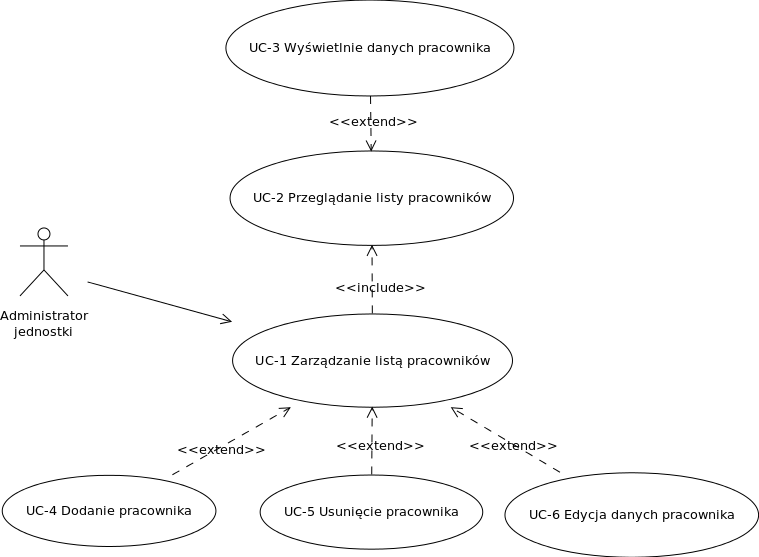
\includegraphics[scale=.6]{img/diagram-uc.png}
	\caption{Diagram przypadków użycia dla zarządzania listą pracowników}
	\label{diagram-uc}
    \end{center}
\end{figure}


\subsection[Scenariusze przypadków użycia][Scenariusze przypadków użycia]{Scenariusze przypadków użycia}
Więcej informacji o poszczególnych funkcjonalnościach system dostarczają scenariusze przypadków użycia. Opisują one w sposób słowny aktorów biorących udział w danych przypadku oraz warunki wstępne oraz końcowe. Opisują też szczegółowo interakcję pomiędzy użytkownikiem a systemem. Wyróżnić można dwie formy takiego opisu: opis w postaci ciągłego tekstu oraz listę kroków. Poniżej przykładowy scenariusz dla przypadku dodawania pracownika:

\paragraph{UC-4 Dodawanie pracownika}
rozszerza UC-1 zarządzanie listą pracowników.\\
\begin{tabular}{ll}
	\textbf{Aktorzy:} & Administrator jednostki \\
	
	\textbf{Warunek początkowy:} & Użytkownik zalogowany w systemie \\
	\textbf{Warunek końcowy:} & Nowy pracownik zapisany w systemie \\
	\multicolumn{2}{l}{\textbf{Scenariusz głowny:}}\\
	\multicolumn{2}{l}{
	\begin{minipage}{\textwidth}\begin{enumerate}
		\item Użytkownik wybiera opcję "Dodaj nowego pracownika".
		\item System wyświetla formularz dadawania użytkownika.
		\item Użytkownik wypełnia formularz.
		\item Użytkownik potwierdza przesłanie formularza przyciskiem "Wprowadź".
		\item System sprawdza poprawność wprowadzonych danych.
		\item System zapisuje dane nowego pracownika
	\end{enumerate}\end{minipage}
	}
\end{tabular}
	
\section[Prototypowanie][Prototypowanie]{Prototypowanie}
Ostatnim etapem fazy analizy jest stworzenie makiet realizowanego systemu. Makiety nie odzwierciedlają faktycznego wyglądu aplikacji, zawierają jednak wszystkie jej elementy w postaci uproszczonych kontrolek. Pozwalają na szersze spojrzenie na całość projektowanego systemu co niekiedy może prowadzić do wychwycenia błędów w jej modelu logicznym. Makiety są wreszcie cenną pomocą dla programistów mających mniejsze doświadczenie w pracy nad częścią kliencką aplikacji. Na rysunku \ref{makieta} przedstawiono przykład makiety formularza do wprowadzania danych pracowników. Została ona wygenerowana za pomocą programu Pencil.

\begin{figure}[tdh]
    \begin{center}
	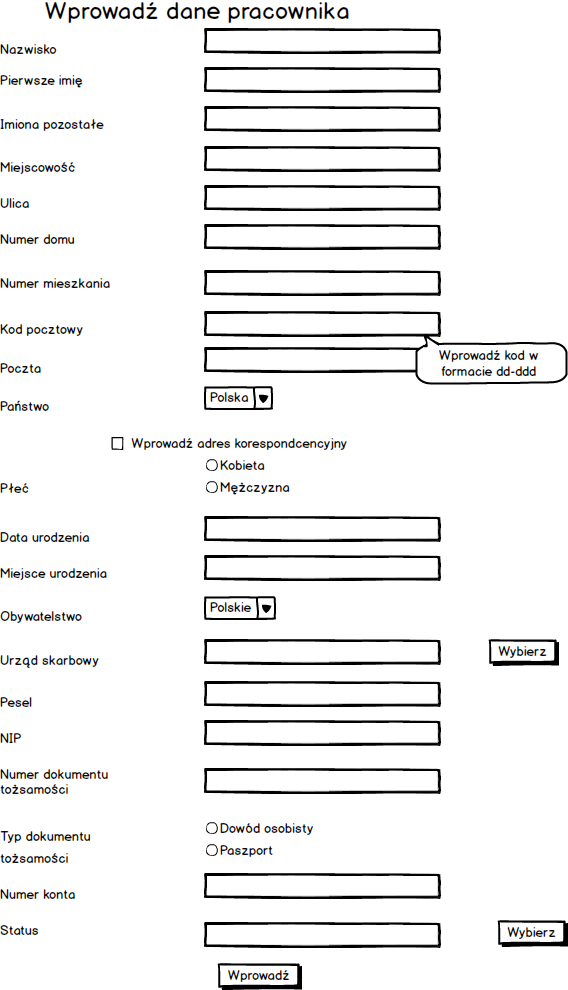
\includegraphics[scale=.8 ]{img/makieta.png}
	\caption{Makieta formularza do wprowadzania danych pracowników}
	\label{makieta}
    \end{center}
\end{figure}

\chapter{Technologie wykorzystane w aplikacji}
\label{chap4}
Poniższy rozdział opisuje wewnętrzną architekturę aplikacji. Zwraca uwagę na jej wielowarstwowy charakter. Dla każdej z warstw opisuje technologie, w których dana warstwa może być realizowana, zwracając szczególną uwagę na te, które zostały wybrane do jej faktycznej implementacji.

\section[Aplikacja w architekturze wielowarstwowej][Aplikacja w architekturze wielowarstwowej]{Aplikacja w architekturze wielowarstwowej}
Podział systemu na warstwy pozwala na ułatwienia w całym cyklu życia aplikacji. W szczególności zmniejsza koszty jego modyfikacji, gdyż wprowadzane zmiany ograniczają się zazwyczaj tylko do jednej warstwy. 

Najprostszym przykładem wielowarstwowej architektury aplikacji jest model typu klient-serwer. Wyróżnia on dwie warstwy:
\begin{itemize}
	\item klienta, stronę żądającą dostępu do jakiejś usługi bądź zasobu,
	\item serwera, stronę udostępniająca daną usługę lub zasób.
\end{itemize}
Architektura ta, dobrze sprawdzająca w małych systemach, zaczęła sprawiać problemy wraz z rozrastaniem się logik biznesowych aplikacji. Efektem tego było pojawienie się pojęć cienkiego i grubego klienta (ang. \textit{thin client} i \textit{fat client}) dla określenia technik umieszczających logikę biznesową po jednej lub po drugiej stronie.

Ostatecznie projektanci systemów wydzielili jeszcze jedną warstwę (odpowiedzialną za realizację logiki biznesowej), doprowadzając do powstania architektury trójwarstwowej. Wyróżnia ona następujące warstwy:
\begin{itemize}
	\item warstwę prezentacji widoczną dla klienta,
	\item warstwę aplikacji realizującą logikę biznesową,
	\item warstwę źródła danych.
\end{itemize}
Rysunek \ref{warstwy} przestawia ogólny schemat aplikacji trójwarstwowej.

\begin{figure}[tdh]
    \begin{center}
	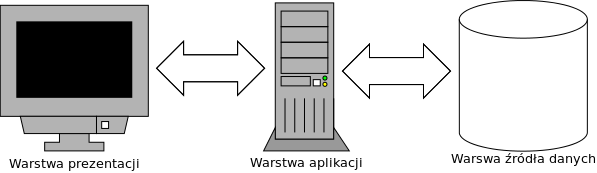
\includegraphics[scale=.7 ]{img/warstwy.png}
	\caption{Schemat komunikacji w architekturze trójwarstwowej}
	\label{warstwy}
    \end{center}
\end{figure}


\section[Warstwa prezentacji][Warstwa prezentacji]{Warstwa prezentacji}
Warstwa prezentacji stanowi interfejs miedzy użytkownikiem a systemem. Najbardziej podstawową implementacją tej warstwy jest terminal znakowy. Funkcje taką może pełnić również aplikacja okienkowa. W przypadku aplikacji webowych warstwa ta realizowana jest w przeglądarce internetowej za pomocą typowych technologii (takich jak HTML, CSS czy JavaScript).

\subsection[HTML][HTML]{HTML}
Podstawową technologią wykorzystywaną do tworzenia widoków aplikacji internetowych jest język znaczników HTML (ang. \textit{Hypertext Markup Language}). Najważniejszą jego zaletą jest przenośność. Zyskujemy dzięki temu niezależność interfejsu od środowiska użytkownika. Niestety sposób prezentacji wciąż jednak zależy (w niewielkim stopniu) od przeglądarki. Jednym z etapów projektu powinno więc być założenie jakie przeglądarki i od jakich wersji będą przez nas wspieranie. Należy też pamiętać, że standard HTML również podlega wersjonowaniu, co oznacza konieczność upewnienia się, czy wpierana przez nas przeglądarka obsługuje HTML w jego najnowszej - piątej wersji. W przeciwnym wypadku musimy ograniczyć się do funkcjonalności z edycji wcześniejszych.

Kolejną zaletą języka znaczników jest jego prostota. Dzięki niej nawet początkujący web-designerzy są w stanie szybko nauczyć się pisania kodu HTML.

Wadą języka HTML jest jego statyczność. Nawet najmniejsza zmiana na stronie wymaga ponownego wygenerowania żądania HTTP i przesłania go do serwera. Wpływa to negatywnie na responsywność aplikacji, szczególnie przy dużym obciążeniu. 
%Zdanie z SDI troche bez sensu ale mozna podrasowac
%Rozwiązaniem tego problemu są technologie takie jak np. AJAX, które generują kod wykonywany na poziomie przeglądarki, bez konieczności ponownego przesyłania żądania.

\subsection[CSS][CSS]{CSS}
W języku HTML możliwe jest wskazanie sposobu wyświetlania informacji. Zaleca się jednak, aby treść dokumentu była odseparowana od sposobu jej prezentacji. Umożliwiają to kaskadowe arkusze stylów (CCS). Pozwalają one na wydzielenie opisu sposobu prezentacji do specjalnych plików. Dzięki zastosowaniu tzw. selektorów możliwe jest zdefiniowanie jednolitego stylu dla całej aplikacji. Łatwiejsze staje się też zarządzanie jej wyglądem.

\subsection[JavaScript][JavaScript]{JavaScript}
JavaScript jest językiem skryptowym wykonywanym po stronie przeglądarki. Pozwala na częściowe ominięcie problemu statyczności dokumentu HTML. Zastosowanie JavaScriptu pozwala osiągnąć większą responsywność stron internetowych. Do typowych jego zastosowań należy obsługa dynamicznych elementów aplikacji (takich jak okna dialogowe) czy wstępna walidacja formularzy. Za pomocą JavaScriptu możemy też manipulować drzewem DOM dokumentu HTML.

\subsection[AJAX][AJAX]{AJAX}
\label{AJAX}
AJAX (ang. \textit{Asynchronous JavaScript and XML}) jest to wieloelementowa technologia pozwalająca na tworzenie kodu wykonującego się w całości po stronie klienta, bez konieczności przeładowywania stron. Daje ona możliwość wysyłania asynchronicznych zapytań do serwera. Pozwala to rozwiązać problem statyczności kodu HTML i daje możliwość tworzenia stron w pełni dynamicznych. Rozwiązanie to ma jednak kilka wad:
\begin{itemize}
	\item utrudnione zarządzanie historią w przeglądarce (mechanizmy pozwalające rozwiązać ten problem pojawiły dopiero w HTML5),
	\item brak możliwości indeksowania treści pobieranych za pomocą żądań AJAX. 
\end{itemize}
Oprócz wspomnianych wcześniej HTML'a, CSS'a i JavaScriptu w skład technologii AJAX wchodzą również:
\begin{itemize}
	\item XMLHttpRequest, klasa umożliwiająca asynchroniczne przesyłanie danych,
	\item XML (ang. \textit{Extensible Markup Language}), język znaczników pozwalający na przesyłanie informacji między klientem a serwerem (obecnie wykorzystuje się również nowsze typy danych np. JSON (ang. \textit{JavaScript Object Notation})).
\end{itemize}
Oczywiście korzystanie z AJAX'a nie zmusza programisty do rezygnacji z tradycyjnych żądań HTTP. Bardzo często można spotkać aplikacje, które większość swoich zapytań realizują synchronicznie, a asynchroniczne zapytania wykorzystują jedynie tam, gdzie ma znaczenie responsywność aplikacji.

\subsection[Dojo Toolkit][Dojo Toolkit]{Dojo Toolkit}
Dojo Toolkit jest zestawem narzędzi opartym na języku JavaScript. Składa się on z trzech podstawowych pakietów.

\subsubsection[dojo][dojo]{dojo}
Jest to główna część zestawu narzędziowego Dojo Toolkit. Zawiera ona najbardziej ogólne moduły pozwalające na komunikację z serwerem za pomocą technologii AJAX, manipulację drzewem DOM czy biblioteki służące do internacjonalizacji.

\subsubsection[dijit][dijit]{dijit}
Jest to zestaw standardowych komponentów interfejsu użytkownika tzw. widżetów (ang. \textit{widgets}) zbudowanych z wykorzystaniem narzędzi z pakietu dojo. Zawiera elementy takie jak np. okna dialogowe czy tooltipy. Na wyróżnienie zasługuje pakiet dijit.form zawierający elementy do budowy i walidacji formularzy.
 
\subsubsection[dojox][dojox]{dojox}
Jest to zestaw skomplikowanych widżetów i funkcji, zbudowanych na podstawie pakietów dojo i dijit. Pozwalają między innymi na tworzenie zaawansowanych efektów graficznych czy wizualizacje danych w postaci wykresów.
 
\section[Warstwa aplikacji][Warstwa aplikacji]{Warstwa aplikacji}
Warstwa aplikacji bywa też czasem nazywana warstwą logiki biznesowej. Jej podstawowym zadaniem jest pośredniczenie pomiędzy warstwą prezentacji a warstwą źródła danych. Odpowiada ona zarówno za odczyt i zapis danych, jak i za ich przekazywanie do wyświetlenia przez użytkownika. Realizuje przy tym często skomplikowaną logikę biznesową.

\subsection[Język programowania][Język programowania]{Język programowania}
Podstawową decyzją jaką musi dokonać projektant systemu jest wybór języka programowania. Determinuje on późniejszy wybór bibliotek, jakie zostaną użyte do tworzenia aplikacji. Ma też wpływ na komfort pracy deweloperów.

\subsubsection{Java}
Java jest językiem w pełni obiektowym. Do swojego działania potrzebuje maszyny wirtualnej, która jest dostępna dla większości (o ile nie dla wszystkich) obecnie spotykanych systemów operacyjnych. Zapewnia to przenośność napisanych w niej aplikacji. Istnieje mnóstwo bibliotek ułatwiających pracę w tym języku, z których większość jest dostępna bezpłatnie. Sam język jest rozwijany przez Oracle Corporation, który wykupił jego oryginalnego twórcę - Sun Microsystems.

\subsubsection{JEE}
Java Enterprise Edition jest rozszerzeniem standardowej platformy języka Java (tzw. Java Standard Edition). Przeznaczona jest ona do tworzenia aplikacji korporacyjnych. Podstawowym założeniem tej platformy jest osadzenie komponentów biznesowych na tzw. serwerze aplikacji (przykładem takiego serwera jest Apache Tomcat). Standardowym zadaniem serwera aplikacji jest praca na poziomie żądań HTTP (ang. \textit{Hypertext Transfer Protocol}), tzn. obsługa żądań oraz wysyłanie odpowiedzi. Zapewnia on także przechowywanie zmiennych sesyjnych 

\subsubsection{C\#}
Podobne funkcje jak Java może pełnić język C\# firmy Microsoft. Dzięki środowisku .NET nadaje się również do tworzenia aplikacji internetowych. Pomimo, iż twórca języka zapewnia o jego przenośności, nie działa on poprawnie na systemach spoza rodziny Windows. Na rynku jest sporo narzędzi ułatwiających programowanie w tym języku. Niestety, są one w większości płatne.

\subsection[Serwlety][Serwlety]{Serwlety}
Podstawowym komponentem realizującym założenia jakie stawia standard JEE jest serwlet. Wszystkie elementy, z których korzystamy tworząc aplikacje webowe (np. strony jsp) są zawsze ostatecznie kompilowane do postaci serwletów. Również frameworki służące do budowania aplikacji internetowych bazują na serwletach.

W ogólności, serwlet nie jest niczym innym jak klasą Javy implementująca interfejs Servlet. W praktyce spotyka się częściej serwlety dziedziczące z abstrakcyjnej klasy HttpServlet. Typowym działaniem takiego serwletu jest obsługa żądań HTTP oraz generowanie odpowiedzi. Zarówno żądanie jak i odpowiedź są oczywiście obudowane w odpowiednie klasy, ale o to dba już sam serwer aplikacji. Zadaniem serwera jest również przekazanie żądania do serwletu (wywołanie jego odpowiedniej metody) jak i odesłanie zwróconej przez serwlet odpowiedzi.

\subsection[ObjectLedge][ObjectLedge]{ObjectLedge}
ObjectLedge jest szkieletem aplikacyjnym (ang. \textit{framework}) bazującym na mechanizmie serwletów. Upraszcza on tworzenie aplikacji internetowych dostarczając szeregu narzędzi do realizacji typowych zadań. W jego skład wchodzi kilka modułów.

\subsubsection{Ledge Web}
Moduł Ledge Web służy do realizacji mechanizmu komunikacji użytkownika z systemem. Opiera się na wzorcu MVC (ang. \textit{Model-View-Controller}). Wzorzec ten polega on odseparowaniu od siebie elementów związanych z logiką biznesową oraz dostępem do danych od elementów związanych z widokiem. Najważniej cechą omawianego modułu jest potokowe przetwarzanie informacji. Programista sam określa sekwencje działań za pomocą tzw. zaworów (ang. \textit{Valve}). Do najważniejszych zadań zaworów należą:
\begin{itemize}
	\item obsługa akcji - zadań niemających bezpośredniego wpływu na widok, ale stanowiących efekt uboczny wykonania żądania,
	\item przygotowanie widoku - części widocznej dla użytkownika.
\end{itemize}
Typowym przykładem potoku jest podział zaworów na 3 klauzule try-catch-finally, gdzie w bloku try umieszczamy zawory odpowiedzialne m. in. za pobranie parametrów zapytania HTTP, obsługę akcji, czy przygotowanie widoku, w bloku catch zawory odpowiedzialne za obsługę sytuacji wyjątkowych (też przygotowujące widok informujący o zaistnieniu takiej sytuacji), zaś w klauzuli finally zawory odpowiadające za przesłanie odpowiedzi do użytkownika.

Obsługę akcji zapewnia zawór o nazwie ActionExecutorValve. Zadaniem programisty jest jedynie zdefiniowanie klasy określającej, co ma zostać wykonane w ramach akcji oraz umieszczenie jej w odpowiedniej strukturze katalogów. Za odnalezienie i wykonanie akcji odpowiada już mechanizm MVC.

Do obsługi widoków wykorzystywany jest zawór BuilderExecutorValve. Pozwala on na ich definiowanie za pomocą odpowiednich klas Javy oraz mechanizmu Velocity (opisanego w dalszej części rozdziału).

\subsubsection{Ledge Intake}
\label{intake}
Moduł ten pozwala na realizację dwóch podstawowych zadań:
\begin{itemize}
	\item konwersji formularzy wprowadzanych przez użytkownika na obiekty języka Java,
	\item walidacji wprowadzanych formularzy.
\end{itemize}
Pierwsze z nich realizowane jest przez zdefiniowanie powiązań pomiędzy polami formularza a właściwościami (ang. \textit{property}) obiektów javowych. Drugie z zadań odbywa się przez zdefiniowanie cech jakie powinny spełniać poszczególne pola formularza. Cechami takimi mogą być między innymi: wartość minimalna czy maksymalna,  format zapisu liczbowego, wyrażenie regularne lub informacja, czy dane pole jest wymagane. Dla każdej z tych cech możliwe jest zdefiniowanie komunikatów, jakie powinny być wyświetlane jeśli dana cecha nie jest spełniona. Do szczególnych zalet modułu Intake należy mocne wsparcie dla internacjonalizacji.

\subsubsection{Ledge Container}
Moduł ten pozwala na zarządzanie zależnościami pomiędzy komponentami programu poza jego kodem. Polega to na zdefiniowaniu klas oraz powiązań między nimi w specjalnym pliku xml. Dzięki temu zależności stają się dynamiczne tzn. nie są definiowane statycznie w momencie kompilacji, ale ustalane są dopiero w momencie wykonania. Pozwala to na zmianę zachowania programu bez konieczności jego rekompilacji (na przykład na zmianę klasy implementującej jakiś interfejs). Takie podejście nazywamy odwróceniem sterowania (ang. \textit{Inversion-of-Control}, w skrócie IoC). Dynamiczne powiązania obiektów możliwe są dzięki mechanizmowi wstrzykiwania zależności (ang. \textit{Dependency Injection}). LegdeContainer bazujący na narzędzi PicoContainer wykorzystuje wstrzykiwanie zależności przez konstruktor. Oznacza to, że wszystkie zależności danego obiektu powinny być argumentami jego konstruktora. Innym przykładem wstrzykiwania zależności jest np. wstrzykiwanie zależności przez metodę ustawiającą (ang. \textit{setter}) popularne w frameworku Spring. Do przechowywania obiektów służy tzw. Kontener. Odpowiada on m. in. za ich poprawną inicjalizację (ustalenie argumentów i przekazanie ich do konstruktora) na początku działania aplikacji.

\subsubsection{Ledge Security}
\label{security}
Moduł ten pozwala na realizację 2 podstawowych zadań stawianych systemom bezpieczeństwa: uwierzytelniania i autoryzacji.

\paragraph{Uwierzytelnianie} polega na sprawdzeniu tożsamości użytkownika, tzn. zweryfikowania czy użytkownik jest rzeczywiście tym, za kogo się podaje. Moduł bezpieczeństwa pozwala na uwierzytelnianie za pomocą nazwy użytkownika i hasła. Warto zaznaczyć, że hasła nie są przechowywane w postaci jawnej, ale w postaci ich funkcji skrótu (przykładem takiej funkcji jest MD5). Uniemożliwia to wejście w posiadanie haseł ani administratorom systemu ani też osobą, które w jakiś (być może niezgodny z prawem) sposób uzyskają dostęp do bazy danych. Oczywiście programista nie jest zmuszony do korzystania z tej postaci uwierzytelniania (wszystko zależy od tego, w jaki sposób zdefiniuje akcję logującą). Możliwe jest m. in. skorzystanie z zewnętrznego systemu służącego do identyfikacji takiego jak LDAP (ang. \textit{Lightweight Directory Access Protocol}, przykładem jego implementacji jest Active Directory firmy Microsoft).

\paragraph{Autoryzacja} polega na przydzieleniu (uwierzytelnionemu wcześniej) użytkownikowi uprawnień do wykonania określonych czynności na określonych obiektach. Mechanizm ten jest w ObjectLedge'u bardzo rozbudowany. Pozwalana on na dynamiczne tworzenie grup zasobów. Mogą być one powiązane z jakąś klasą obiektów, bądź z ich konkretnymi instancjami. W ramach grup użytkownikom przydzielane są role. Role zaś wiążą się z konkretnymi pozwoleniami (ang. \textit{permission}). Pozwolenia te określą dostęp do poszczególnych widoków, akcji oraz wywołań AJAX w ramach danej grupy zasobów.

\subsection[Apache Velocity][Apache Velocity]{Apache Velocity}
\label{velocity}
Velocity jest mechanizmem szablonów pozwalającym na szybkie tworzenie dokumentów. W przypadku aplikacji webowych są to zazwyczaj dokumenty HTML, co jednak nie jest regułą. Velocity jest też powszechnie wykorzystywane do tworzenia dokumentów w standardzie XML i jego pochodnych (np. XHTML czy VoiceXML). Najważniejszą cechą tego mechanizmu jest to, że został on w całości napisany w Javie. Pozwala to na odwoływanie się z poziomu kodu szablonów bezpośrednio do obiektów tego języka. Pozwala on również na definiowanie zmiennych, instrukcji warunkowych oraz pętli za pomocą odpowiednich makr, a także na dodawanie makr zdefiniowanych przez programistę.

\subsection[Spring Framework][Spring Framework]{Spring Framework}
Spring, podobnie jak ObjectLedge, jest szkieletem aplikacyjnym przeznaczonym dla platformy Java/JEE. Składa się on z kilku niezależnych modułów. Do najważniejszych z nich należą:
\begin{itemize}
	\item kontener IoC, 
	\item szablon programowania aspektowego,
	\item szablon dostępu do danych,
	\item szablon zarządzania transakcjami,
	\item szablon MVC,
	\item szablon bezpieczeństwa.
\end{itemize}
Niestety, duża ilość komponentów wpływa negatywnie na wydajność. Powoduje to powolną migrację programistów w stronę innych frameworków. Mimo to, Spring jest ciągle najpopularniejszym narzędziem tego typu.

%\subsection[Java Server Pages][Java Server Pages]{Java Server Pages}
%TODO jako alternatywa dla Velocity

\subsection[JDBC][JDBC]{JDBC}
JDBC (ang. \textit{Java DataBase Connectivity}, częśc platformy Java Standard Edition) jest interfejsem pozwalającym na wykonywanie zapytań SQL z poziomu języka Java. Do poprawnego działania wymaga sterownika bazy danych, z którą ma współpracować. Niestety korzystanie z niego bezpośrednio w aplikacji jest uciążliwe, a stąd rzadko spotykane. Służy jednak jako podstawa do bardziej zaawansowanych narzędzi realizujących dostęp do warstwy danych. Najprostszym przykładem takiego narzędzia jest JdbcTemplate z frameworka Spring. Z JDBC korzystają również narzędzia służące do mapowania obiektowo-relacyjnego (ang. \textit{object-relational mapping}, w skrócie ORM) takie jak Hibernate.

\subsection[Hibernate][Hibernate]{Hibernate}
\label{hibernate}
Hibernate jest obecnie najpopularniejszym frameworkiem pozwalającym na implementację warstwy dostępu do danych (ang. \textit{persistence layer}). Został on stworzony z myślą o języku Java, istnieje jednak jego wersja dla środowiska .NET (tzw. NHibernate).

Podstawowym zadaniem jakie spełnia Hibernate jest odwzorowanie struktury obiektów języka Java na relacyjną bazę danych, zwane mapowaniem obiektowo-relacyjnym. Odwzorowania tego można dokonać na dwa sposoby:
\begin{itemize}
	\item z wykorzystaniem plików hbm.xml,
	\item za pomocą adnotacji JPA (Java Persistence API).
\end{itemize}

Pliki hbm.xml (ang. \textit{Hibernate Mapping files}) są podstawowym sposobem realizacji mapowania obiektowo-relacyjnego w Hibernate. Mają one format dokumentów xml zawierających informacje o sposobie, w jaki dane z tabel relacyjnych mają być tłumaczone na obiekty domenowe. Do najważniejszych z nich należą: nazwa tabeli oraz kwalifikowana nazwa klasy, informacje o kluczu głównym, nazwy kolumn tabeli i właściwości (niekoniecznie pól) klasy czy  informacje o relacjach z innymi tabelami (również odwzorowywanymi w strukturze obiektowej). Nie ma ograniczenia na liczbę klas, które można zmapować za pomocą jednego pliku, zaleca się jednak, aby mapowanie każdej klasy znajdowało się w osobnym dokumencie. Istnieją narzędzia pozwalające na automatyczną generację klas domenowych oraz plików hbm.xml na podstawie struktury bazy danych. Jednym z nich jest Hibernate Tools, będący częścią projektu Hibernate.

Java Persistence API jest oficjalnym standardem języka Java służącym do mapowania obiektowo-relacyjnego. Standard ten jest implementowany nie tylko przez Hibernate, ale też przez inne ORM-y, co umożliwia zmianę narzędzia bez konieczności przebudowy dużej części aplikacji. Założeniem JPA jest wykorzystanie specjalnie przygotowanych adnotacji języka Java bezpośrednio w kodzie klas, które mają być odwzorowane na tabele. Pozwala to zwiększyć czytelność kodu, sprawiając, że zarówno klasa jak i jej mapowanie znajdują się w jednym pliku. Wadą tego rozwiązania są mniejsze możliwości niż plików hbm.xml. Pamiętać także należy, że adnotacje pojawiły się w Javie dopiero w wersji 1.5, co może okazać się kłopotliwe w przypadku korzystania ze starszych wersji oprogramowania.

Hinernate oferuje również bazujący na SQL język - HQL (ang. \textit{Hibernate Query Language }). Pozwala on na tworzenie zapytań z wykorzystaniem obiektów domenowych. Zaletą tego rozwiązania jest to, że niewielkie zmiany w bazie danych (np. zmiana nazwy tabeli bądź kolumny) nie muszą oznaczać konieczności zmian zapytań HQL.

\section[Warstwa źródła danych][Warstwa źródła danych]{Warstwa źródła danych}
Najważniejszym elementem aplikacji jest system zarządzania bazą danych (ang. \textit{Database Management System}, w skrócie DBMS). Jako jedyny jest prawie niemożliwy do wymiany. Decyzja o jego wyborze powinna być starannie przemyślana, gdyż może stanowić o przyszłym powodzeniu lub klęsce całego systemu.

\subsection[Oracle Database 11g Express Edition][Oracle Database 11g Express Edition]{Oracle Database 11g Express Edition} 
Niekwestionowanym liderem rynku systemów zarządzania bazą danych jest firma Oracle ze swoim produktem zwanym Oracle Database. Niestety większość jego wersji (takich jak np. Oracle Database Enterprise Edition) jest płatna. Bezpłatnie dostępna jest jedynie wersja Express Edition oznaczona numerem 11g (najnowsza edycja 12c dostępna jest tylko w wersjach płatnych).  Posiada ona jednak istotne ograniczenia. Do podstawowych z nich należą:
\begin{itemize}
	\item wykorzystanie mocy obliczeniowej co najwyżej jednego procesora,
	\item ograniczenie wykorzystania pamięci RAM do 1GB,
	\item ograniczenie rozmiaru bazy danych do 11GB,
	\item brak wsparcia technicznego.
\end{itemize}

\subsection[MySQL][MySQL]{MySQL} 
MySQL jest prawdopodobnie najpopularniejszym darmowym systemem zarządzania bazą danych. Szczególnie chętnie bywa łączony z technologiami takimi jak PHP, służąc do budowy stron internetowych oraz prostych aplikacji webowych. W śród deweloperów krąży jednak wiele negatywnych opinii na jego temat. Od 2010 roku jest rozwijany przez firmę Oracle.

\subsection[PostgreSQL][PostgreSQL]{PostgreSQL} 
PostgreSQL, zwany też po prostu Postgres, jest bardzo zaawansowanym systemem zarządzania bazą dodanych. Jest on następcą nieistniejącego już systemu o nazwie Ingres. Rozpowszechniany jest na zasadzie wolnego oprogramowania na licencji zwanej PostgreSQL, podobnej do licencji BSD. Do jego najważniejszych cech należą:
\begin{itemize}
	\item rozbudowany język proceduralny PL/pgSQL (podobny do PL/SQL używanego w bazach Oracle),
	\item zgodność ze standardem SQL:2008 (implementuje też większość nowszego standardu SQL:2011),
	\item rozszerzona definicja typów (w porównaniu do standardu SQL),
	\item wysoka wydajność (m. in. dzięki zastosowaniu mechanizmu MVCC (ang. \textit{Multiversion Concurrency Control}) do zarządzania transakcjami),
	\item brak ograniczeń na rozmiar bazy danych(istnieją czysto techniczne ograniczenia na wielkość niektórych elementów w bazie, ale są one liczone w terabajtach i nie powinny mieć wpływu na działanie aplikacji),
	\item stabilność działania,
	\item dostępność na większość używanych obecnie systemów operacyjnych (Wiele dystrybucji likuksa zawiera pakiety umożliwiające instalację bazy PostgreSQL, znajdują się one m. in. w repozytorium popularnej dystrybucji Ubuntu),
	\item bogata dokumentacja.
\end{itemize}
Wszystkie te czynniki czynią Postgres jednym z trzech (obok wspomnianego wcześniej MySQL i Firebird) najpopularniejszych systemów zarządzania bazą danych dostępnych za darmo. W 2012 roku został odznaczony tytułem Linux New Media Award for Best Open Source Database.

\section[Narzędzia wspomagające tworzenie aplikacji][Narzędzia wspomagające tworzenie aplikacji]{Narzędzia wspomagające tworzenie aplikacji}

\subsection[Eclipse][Eclipse]{Eclipse}
Eclipse jest popularnym zintegrowanym środowiskiem programistycznym (ang. \textit{Integrated Development Environment}, IDE). Mimo, iż jest ono przeznaczone głównie do tworzenia programów w języku Java, możliwe jest jego wykorzystanie do programowania w różnych językach. Zapewnia to mechanizm wtyczek (ang. \textit{plugin}). Pozwalają one na dowolne rozszerzanie jego funkcjonalności. Umożliwiają one nie tylko wspomaganie programowania w danym języku, ale również tworzenie GUI, modelowanie w UML, współpracę z bazami danych czy serwerami aplikacji. Przykładem aplikacji zbudowanej z platformy Eclipse oraz odpowiedniego zestawu wtyczek jest Rational Software Architect firmy IBM.

\subsection[Maven][Maven]{Maven}
Maven jest narzędziem automatyzującym proces budowy oprogramowania. Budowanie to odbywa się na podstawie opisu projektu zawartego w specjalnym pliku o nazwie pom.xml. Plik taki zawiera najważniejsze informacje o projekcie oraz sposobie jego budowania. Nie zawiera natomiast (w przeciwieństwie np. do Anta) szczegółowego opisu kroków, w jakich miałby przebiegać proces budowy aplikacji. Ważnym elementem takiego pliku są tzw. zależności (ang. \textit{dependency}) - biblioteki wykorzystywane przez tworzoną aplikację. Są one automatycznie pobierane ze zdalnego repozytorium Mavena (bądź innego wskazanego w pliku pom.xml), a następnie umieszczane w lokalnym repozytorium na komputerze programisty. Budowanie aplikacji odbywa się przez osiągnięcie wybranego przez programistę celu. Do najważniejszych z nich należą:
\begin{itemize}
	\item compile - kompilacja kodu źródłowego,
	\item test - uruchomienie testów jednostkowych,
	\item package - budowa tzw. paczki najczęściej w postaci archiwum JAR lub WAR,
	\item install - umieszczenie paczki w lokalnym repozytorium,
	\item deploy - umieszczenie paczki w zdalnej lokalizacji np. na serwerze aplikacji.
\end{itemize}
Wymienione cele są, częścią tzw. głównego cyklu życia projektu. Oznacza to, że w osiągnięcie każdego z nich powinno być poprzedzone realizacją celów znajdujących się na wyższych pozycjach listy.


\chapter{Model danych}
\label{chap5}

\section[Model logiczny][Model logiczny]{Model logiczny}
Jednym z pierwszych etapów projektowania systemów informatycznych jest stworzenie modelu logicznego. Prezentuje on ogólną koncepcję modelu danych, niezwiązaną z żadnym konkretnym systemem zarządzania bazą danych. Najpopularniejszym przykładem modelu logicznego jest model związków encji. Polega on na przedstawieniu zagadnienia za pomocą encji, ich atrybutów oraz związków pomiędzy nimi. Na rysunkach \ref{logiczny1}, \ref{logiczny2}, \ref{logiczny3} przedstawiono diagramy związków encji dla projektowanej aplikacji.

\begin{figure}[tdh]
    \begin{center}
	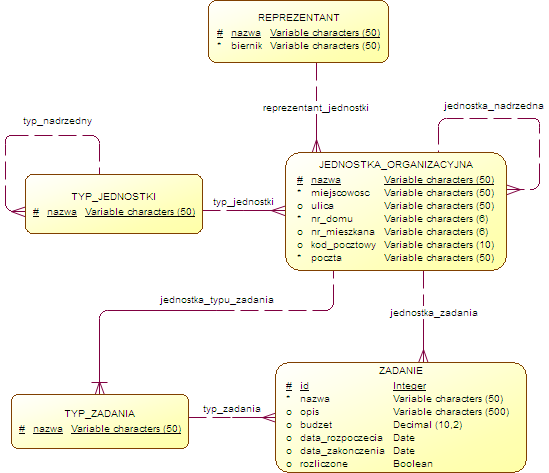
\includegraphics[scale=.8]{img/logiczny1.png}
	\caption{Model związków encji opisujący strukturę organizacyjną instytucji}
	\label{logiczny1}
    \end{center}
\end{figure}
\begin{figure}[tdh]
    \begin{center}
	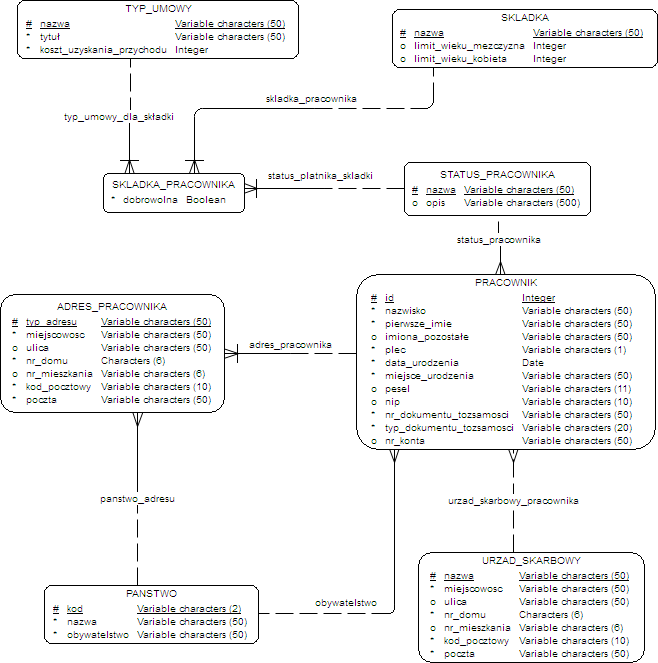
\includegraphics[scale=.8]{img/logiczny2.png}
	\caption{Model związków encji opisujący pracownika}
	\label{logiczny2}
    \end{center}
\end{figure}
\begin{figure}[]
    \begin{center}
	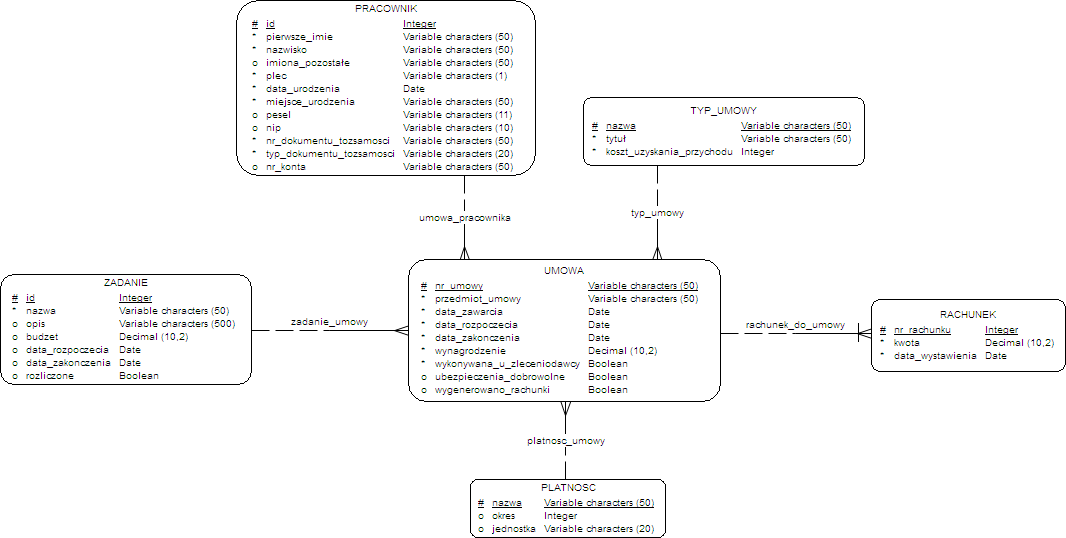
\includegraphics[scale=.8,angle=-90]{img/logiczny3.png}
	\caption{Model związków encji opisujący umowę}
	\label{logiczny3}
    \end{center}
\end{figure}

\subsubsection{Pracownik}
Encja ta zawiera informacje dotyczące pracownika, który może być zatrudniany na umowy-cywilno prawne. Powstała na podstawie wymagań opisanych w rozdziale \ref{pracownicy}. Podstawowymi atrybutami tej encji są nazwisko i imiona pracownika. Imiona opisane zostały dwoma atrybutami: obowiązkowym - pierwsze imię oraz opcjonalnym - imiona pozostałe. Kolejnymi atrybutami pracownika są płeć, data urodzenia, miejsce urodzenia, numery PESEL oraz NIP, numer konta oraz numer dokumentu tożsamości. Dokumentem takim może dowód osobisty lub paszport  (w przypadku obcokrajowców). Powstała więc konieczność wprowadzenia kolejnego atrybutu jakim jest typ dokumentu tożsamości.

W przypadku tej encji nie udało się znaleźć naturalnego identyfikatora. Nie może nim być zbiór atrybutów: nazwisko oraz pierwsze imię, gdyż niewykluczona jest sytuacja, że w systemie znajdzie się dwóch pracowników nazywających się tak samo. Funkcji takiej nie mogą także pełnić numery PESEL oraz NIP. Występują przecież pracownicy nie posiadający takich numerów. Wprowadzono więc sztuczny identyfikator w postaci atrybutu id.

\subsubsection{Adres Pracownika}
Encja ta powstała z konieczności umożliwienia posiadania przez pracownika trzech adresów: 
\begin{itemize}
	\item zameldowania - umieszczanego na umowie,
	\item zamieszkania - wykorzystywanego w celach podatkowych,
	\item korespondencyjnego.
\end{itemize}
Stąd też podstawowym atrybutem tej encji jest typ adresu (zameldowania, zamieszkania, lub korespondencyjny). Oprócz tego posiada takie atrybuty jak miejscowość, ulica, numer domu, numer mieszkania, kod pocztowy i poczta. Na uwagę zasługują atrybuty: ulica i numer mieszkania. Nie są one obowiązkowymi elementami adresu, gdyż ulice nie występują w każdej miejscowości (szczególnie na wsiach, ze względu małą liczbę mieszkańców, nie ma potrzeby ich wprowadzania), a numerów mieszkania nie posiadają m. in. domy jednorodzinne. Kolejną istotną kwestią jest rozdzielenie atrybutów miejscowość i poczta. Wiele modeli niesłusznie zakłada, że atrybuty te są tożsame. Niestety, nie jest to regułą - nie każda miejscowość jest siedzibą poczty.
W przypadku tak skonstruowanej encji udało się znaleźć naturalny identyfikator. Jest to para: związek z encją pracownik oraz atrybut typ adresu.

\subsubsection{Państwo}
Jest to encja słownikowa. Pojawiła się w systemie z dwóch powodów. Pierwszym z nich jest konieczność przechowywania informacji o obywatelstwie pracownika  (stąd związek ,,obywatelstwo''). Drugim powodem jest obecność państwa w adresie. Atrybutami państwa są jego nazwa (np. Polska) oraz nazwa obywatelstwa (np. polskie). Jako unikalny identyfikator państwa wybrano dwuliterowy kod ISO-3166-1\cite{panstwa} (np. PL).

\subsubsection{Urząd Skarbowy}
Encja ta opisuje urząd skarbowy właściwy dla pracownika. Podstawowym jej atrybutem jest nazwa. Pełni ona funkcję unikalnego identyfikatora tej encji. Zawiera ona zazwyczaj informacje o miejscowości oraz numerze urzędu skarbowego (np. Pierwszy Urząd Skarbowy w Lublinie). Nie jest to jednak regułą. Zdarza się, że zamiast numeru występuje nazwa dzielnicy czy nazwa własna urzędu skarbowego. Niemożliwym stało się więc rozbicie tego atrybutu na mniejsze części (w szczególności wyodrębnienie atrybutu numer urzędu skarbowego). Pozostałymi atrybutami urzędu skarbowego są dane adresowe, czyli miejscowość, ulica, numer domu, numer mieszkania, kod pocztowy i poczta.

\subsubsection{Status pracownika}
Encja ta opisuje status pracownika w świetle obowiązków odprowadzania składek na różnego rodzaju ubezpieczenia i fundusze. Przykłady takich statusów zostały opisane w sekcji \ref{przykladyOsob}. Atrybutami tej encji są nazwa oraz opis. Nazwa jest ponadto jej unikalnym identyfikatorem.

\subsubsection{Jednostka organizacyjna}
Encja ta powstała w celu odwzorowania hierarchicznej struktury instytucji. Cechą wyróżniającą ją z pośród innych encji jest związek rekurencyjny. Dla każdej jednostki definiuje on jednostkę nadrzędną w stosunku do niej. Związek taki jest oczywiście obustronnie opcjonalny (w przeciwnym wypadku nie dałoby się zamodelować jednostek będących liśćmi w drzewie hierarchii, a także jego korzenia). Do atrybutów jednostki należy nazwa (będąca jej unikalnym identyfikatorem) oraz jej dane adresowe, czyli miejscowość, ulica, numer domu, numer mieszkania, kod pocztowy i poczta.

\subsubsection{Typ jednostki}
Kolejna encja słownikowa. Jej jedynym atrybutem i zarazem unikalnym identyfikatorem jest nazwa. Podobnie jak jednostka organizacyjna posiada związek rekurencyjny definiujący typ nadrzędny. Dzięki temu już samo sprawdzenie typów jednostek pozwala zapewnić acykliczność w strukturze organizacji.

\subsubsection{Reprezentant}
Reprezentant jednostki. W imieniu jednostki podpisuje on umowy. Informacja o nim powinna się też znaleźć w części umowy definiującej strony  (np. Jednostka X reprezentowana przez ...). W tym przypadku zdecydowano się nie wydzielać osobnych atrybutów takich jak imię czy nazwisko, a pozostać przy jednym atrybucie nazwa (stała się ona unikalnym identyfikatorem tej encji). Ważniejszym okazało się przechowywanie jej formy biernika, która okazała się potrzeba w celu umieszczenia jej na umowie.

\subsubsection{Zadanie}
Zadanie wykonywane w ramach jednostki. Jego jedynym obowiązkowym atrybutem jest nazwa. Posiada też atrybuty opcjonalne: opis, budżet, daty rozpoczęcia i zakończenia oraz informację czy zostało ono rozliczone. W przypadku zadania nazwa nie może pełnić funkcji unikalnego identyfikatora. W systemie może przecież istnieć kilka zadań o tej samej nazwie. Kandydatem na unikalny identyfikator wydaje zestaw trzech elementów: nazwy oraz związków z encjami jednostka organizacyjna i typ zadania. Niestety taki identyfikator jest zbyt duży, stąd już na tym etapie zdecydowano się na wprowadzenie sztucznego identyfikatora w postaci atrybutu id.

\subsubsection{Typ zadania}
Encja powstała w celu pogrupowania zadań w ramach jednostki. Jedynym jej atrybutem jest nazwa. Wchodzi ona, wraz ze związkiem z jednostką organizacyjną w skład unikalnego identyfikatora encji.

\subsubsection{Umowa}
Jedna z najważniejszych encji w systemie. Łączy pracownika z zadaniem. Zawiera atrybuty takie jak: numer umowy, przedmiot umowy, daty zawarcia, rozpoczęcia i zakończenia, wynagrodzenie, informacje czy jest wykonywana u zleceniodawcy, czy pracownik chce z jej tytułu przystąpić do ubezpieczeń dobrowolnych oraz czy wszystkie rachunki do umowy zostały już wygenerowane przez system. Numer umowy jest nadawany przez system w celu jej łatwiejszej identyfikacji. Powstaje on z połączenia daty zawarcia umowy oraz numeru umowy w danym dniu. Ma on więc cechy zarówno identyfikatora naturalnego jak i sztucznego. Atrybut mówiący o tym czy wszystkie rachunki do umowy zostały już wygenerowane nie jest widoczny dla użytkownika. Nie był on także uwzględniony w fazie analizy. Pojawił się dopiero w fazie implementacji. Wykorzystywany jest jedynie przez mechanizm generujący rachunki do umowy.

\subsubsection{Płatność}
Encja ta opisuje sposób płatności z tytułu umowy, może on być jednorazowy lub ratalny. W przypadku tego drugiego konieczne jest zdefiniowanie okresu, co jaki mają być wypłacane raty. Służą do tego atrybuty okres oraz jednostka okresu. Pierwszy z nich oznacza liczbę dni lub miesięcy, co które ma być wypłacane wynagrodzenie. Drugi przyjmuje jedną z dwóch wartości wyliczeniowych: dni lub miesiące. Oprócz nich płatność posiada nazwę, która jest jej unikalnym identyfikatorem.

\subsubsection{Rachunek}
Rachunek jest podstawą do wypłacenia wynagrodzenia. Występuje zawsze w związku z umową. Posiada unikalny w skali danej umowy numer. Unikalnym identyfikatorem jest więc para: związek z encją umowa i atrybut numer. Pozostałymi atrybutami tej encji są kwota oraz data wystawienia.

\subsubsection{Typ Umowy}
Encja ta definiuje tytuł umowy oraz koszt uzyskania przychodu. Posiada też nazwę, która jest jej unikalnym identyfikatorem. Nazwa może, ale nie musi, być tożsama z tytułem umowy.

\subsubsection{Składka}
Encja identyfikująca składki na ubezpieczenia społeczne i zdrowotne oraz fundusze celowe. Podstawowym jej atrybutem a zarazem unikalnym identyfikatorem jest nazwa. Odprowadzanie składek na fundusze celowe ograniczone jest limitem wiekowym. Jest on różny dla kobiet i mężczyzn. Można to zamodelować na 2 sposoby. Pierwszy z nich polega na wprowadzeniu atrybutów opisujących limit wieku dla każdej płci. Drugim sposobem jest wprowadzenie dodatkowej encji pozostającej w związku z encją składka, posiadającej atrybuty płeć oraz limit wieku. Ze względu na tylko dwie płcie oraz niezmienność tej cechy postanowiono skorzystać z pierwszego rozwiązania.

\subsubsection{Składka pracownika}
Encja ta jest przykładem realizacji rzadko spotykanego związku trynarnego (związku między trzema encjami).  Łączy ze sobą encje: typ umowy, składka i status pracownika. Połączanie takie oznacza, że pracownik o takim statusie odprowadza taką składkę od umowy o takim typie. Związek taki zawsze jest realizowany przez wprowadzenie dodatkowej encji już na etapie modelu logicznego.  Jest to ponadto podyktowane występowaniem dodatkowej cechy tego związku jakim jest informacja, czy dana składka jest dobrowolna. Jest to encja słaba. Oznacza to, że jej unikalnym identyfikatorem są wszystkie jej związki.


\section[Schemat tabel][Schemat tabel]{Schemat tabel}
\label{modelFizyczny}
Kolejnym etapem pracy nad projektem jest stworzenie schematu tabel. Powstaje on na podstawie modelu logicznego z uwzględnieniem aspektów implementacyjnych. Są nimi między innymi technologie wykorzystywane do tworzenia systemu, w szczególności wybrany przez nas system zarządzania bazą danych. Podstawowymi jego elementami są tabele, ich kolumny oraz klucze obce. Na rysunkach \ref{fizyczny1}, \ref{fizyczny2}, \ref{fizyczny3} przedstawiono schematy tabel projektowanego systemu.



\begin{figure}[tdh]
    \begin{center}
	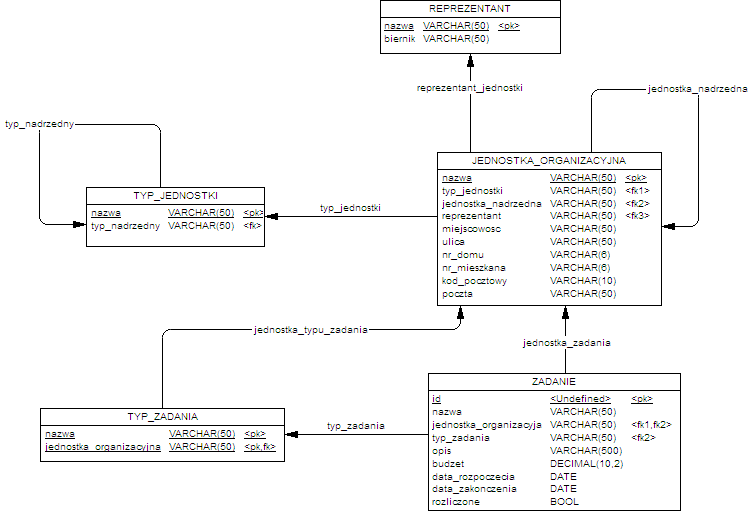
\includegraphics[scale=.8]{img/fizyczny1.png}
	\caption{Schemat tabel opisujący strukturę organizacyjną instytucji}
	\label{fizyczny1}
    \end{center}
\end{figure}
\begin{figure}[tdh]
    \begin{center}
	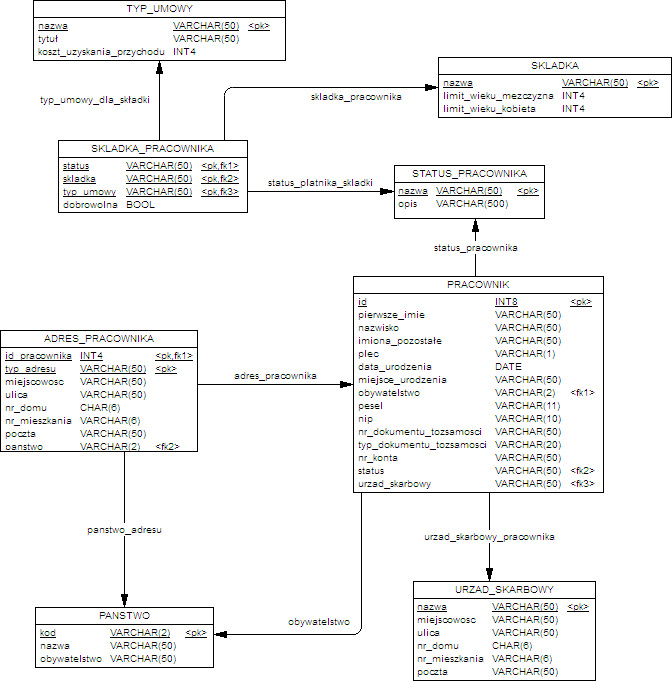
\includegraphics[scale=.8]{img/fizyczny2.png}
	\caption{Schemat tabel opisujący pracownika}
	\label{fizyczny2}
    \end{center}
\end{figure}
\begin{figure}[tdh]
    \begin{center}
	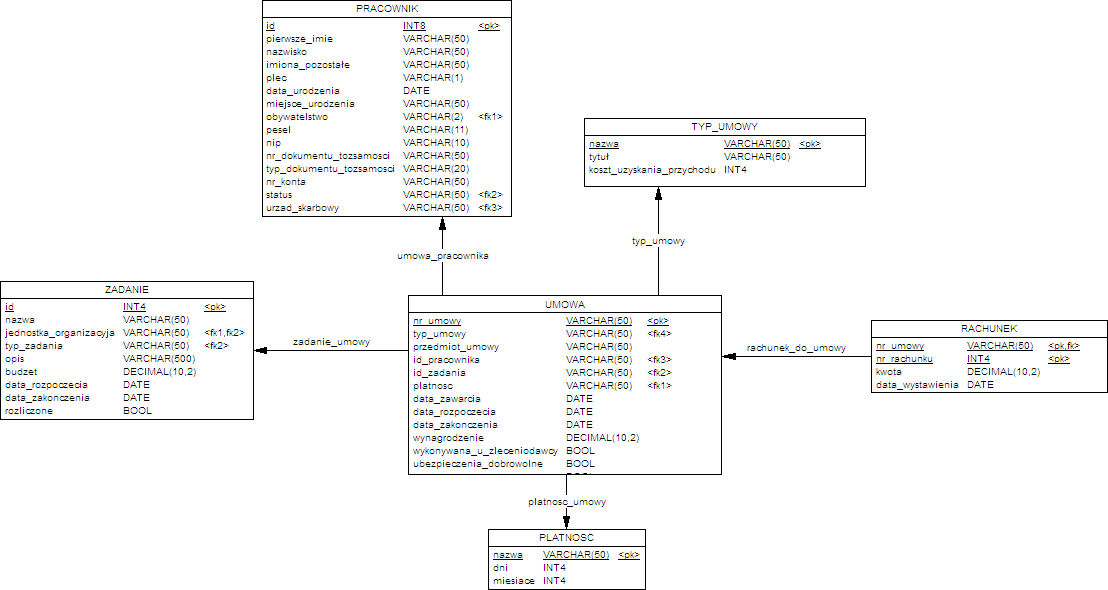
\includegraphics[scale=.8,angle=-90]{img/fizyczny3.png}
	\caption{Schemat tabel opisujący umowę}
	\label{fizyczny3}
    \end{center}
\end{figure}

\subsection[Schemat tabel a diagram ER][Schemat tabel a diagram ER]{Schemat tabel a diagram ER}
W projektowanym systemie nie ma dużych różnic pomiędzy schematem tabel a diagramem związków encji.
Encje zamieniono na tabele, zaś związki na klucze obce. 

\subsection[Wybór kluczy głównych][Wybór kluczy głównych]{Wybór kluczy głównych}
Jako klucze główne posłużyły unikalne identyfikatory encji. Stało się tak również w przypadkach, w których wybór ten oznaczał pojawienie się klucza złożonego. W przypadkach, w których występowały związki identyfikujące, w skład kluczy złożonych weszły klucze obce.

\subsection[Związki wiele do wielu][Związki wiele do wielu]{Związki wiele do wielu}
Standardowym działaniem podczas przejścia z modelu związków encji do schematu tabel jest zamiana binarnych związków wiele do wielu na tabele. W projektowanym systemie takie nie występowały. Pojawił się natomiast związek trynarny. Związki takie są jednak modelowane jako encje już na etapie modelu ER.


\chapter{Implementacja}
\label{chap6}

\section{Baza danych}
Warstwa obiektów trwałych została oparta na systemie PostgreSQL. Schemat danych powstał na podstawie modelu opisanego w rozdziale \ref{modelFizyczny}. Oprócz definicji tabel zawiera on również sekwencje służące do generowania sztucznych kluczy głównych. Dla kolumn zawierających wartości wyliczeniowe (takich jak płeć mogąca przyjmować jedną z 2 wartości) zdefiniowano więzy kontrolne za pomocą klauzul check.

\section{Dostęp do danych}
Dostęp do danych został zrealizowany przy użyciu narzędzia Hibernate z wykorzystaniem wzorca DAO oraz obiektów POJO.

\subsection[Hibernate][Hibernate]{Hibernate} 
Technologa Hibernate została opisana w rozdziale. \ref{hibernate}. Mapowanie obiektowo-relacyjne wykonano przy pomocy plików hbm.xml. Na wydruku \ref{adresHbm} przedstawiono fragment pliku zawierającego mapowanie tabeli Adres pracownika.

\begin{lstlisting}[language=XML,style=outcode,showstringspaces=false, caption=Mapowanie tabeli Adres pracownika w postaci pliku hbm.xml,label={adresHbm}]
<?xml version="1.0"?>
<hibernate-mapping>
	<class name="pl.waw.mizinski.umowy.model.AdresPracownika"
			table="adres_pracownika" lazy="true">
		<composite-id name="adresPracownikaPK" 
				class="pl.waw.mizinski.umowy.model.AdresPracownikaPK">
			<key-many-to-one name="pracownik" 
					class="pl.waw.mizinski.umowy.model.Pracownik">
				<column name="pracownik" sql-type="int4"/>
			</key-many-to-one>
			<key-property name="typAdresu" column="typ_adresu">
				<type name="org.hibernate.type.EnumType">
					<param name="enumClass">
						pl.waw.mizinski.umowy.model.enums.TypAdresu
				</param>
					<param name="type">12</param>
				</type>
			</key-property>
		</composite-id>
		<property name="miejscowosc" type="java.lang.String">
			<column name="miejscowosc" sql-type="varchar" />
		</property>
		
		<!-- ... -->
		
		<many-to-one name="panstwo" class="pl.waw.mizinski.umowy.model.Panstwo">
			<column name="panstwo" />
		</many-to-one>
	</class>
</hibernate-mapping>
\end{lstlisting}

Tabela ta pozwala na posiadanie przez pracownika trzech adresów (zameldowania, zamieszkania i korespondencyjnego). Odzwierciedla to jej klucz główny. Składa się on z klucza obcego, odwzorowanego na klasę Pracownik oraz kolumny typ adresu odwzorowanej na typ wyliczeniowy. 


\subsection[Obiekty DAO][Obiekty DAO]{Obiekty DAO}
%DAO (ang. \textit{Data Access Object} - Obiekt dostępu do danych) jest to wzorzec projektowy polegający na dostarczeniu interfejsu pozwalającego na dostęp oraz manipulację danymi. Obiekty takie tworzą osobną warstwę oddzielającą warstwę logiki biznesowej od warstwy źródła danych. 
W aplikacji skorzystano z wzorca DAO. Wykorzystywane w systemie obiekty DAO dziedziczą z abstrakcyjnej klasy bazowej, definiującej podstawowe operacje jakie można wykonać na obiektach trwałych. Została ona zaprezentowana na wydruku \ref{abstractDao}.

\begin{lstlisting}[language=Java,style=outcode,showstringspaces=false,caption=Bazowa klasa DAO,label={abstractDao}]
public abstract class AbstractDao<K extends Serializable, E> {

	protected final Context context;
	private final Class<E> entityClass;

	public AbstractDao(Context context) {
		this.context = context;
		ParameterizedType genericSuperclass = (ParameterizedType) getClass()
				.getGenericSuperclass();
		this.entityClass = 
				 (Class<E>) genericSuperclass.getActualTypeArguments()[1];
	}

	protected Session session() {
		return HibernateSessionContext.getHibernateSessionContext(context)
				.getSession();
	}

	public Class<E> getEntityClass() {
		return entityClass;
	}

	public E getById(K id) {
		return (E) session().get(getEntityClass(), id);
	}

	public void add(E entity) {
		session().persist(entity);
	}

	public K save(E entity) {
		return (K) session().save(entity);
	}

	public void remove(E entity) {
		session().delete(entity);
	}

	...

}
\end{lstlisting}

Przedstawiona klasa jest klasą generyczną. Parametryzowana jest dwoma typami danych: typem obiektu mapowanego na tabelę oraz typem jego klucza. 

\subsection[Obiekty POJO][Obiekty POJO]{Obiekty POJO}
Oprócz metod dziedziczonych z klasy bazowej, obiekty DAO posiadają też metody służące do odczytu danych w postaci obiektów POJO (ang. \textit{Plain Old Java Object}).
Obiekty takie posiadają jedynie konstruktor oraz metody odczytujące wartości ich pól. Najczęstszym zastosowaniem obiektów POJO w aplikacji jest przekazywanie ich do mechanizmu Velocity w celu przygotowania widoku.

\begin{comment}
Metody bazowej klasy DAO zwracają obiekty trwałe. Powoduje to często niepotrzebny narzut wydajnościowy. Rozwiązaniem tego problemu jest wykorzystanie, niepowiązanych z sesją Hibernate, obiektów POJO (ang. \textit{Plain Old Java Object}). Wydruk \ref{pojo} zawiera metodę DAO zwracającą listę obiektów POJO opisujących umowę. Metoda ta dokonuje złączenia tabel już na etapie zapytania HQL.

\begin{lstlisting}[language=Java,style=outcode,showstringspaces=false,caption=Metoda DAO zwracająca listę obiektów POJO opisujących umowę,label={pojo}]
public class UmowaDao extends AbstractDao<String, Umowa> {

	public static final String SIMPLE_UMOWA_POJO = 
		"pl.waw.mizinski.umowy.pojo.SimpleUmowaPOJO("
		+ "u.nrUmowy, u.typUmowy.nazwa, p.nazwisko, p.pierwszeImie, " +
		"p.imionaPozostale, z.typZadania.typZadaniaPK.jednostkaOrganizacyjna.nazwa,"
		+ "z.nazwa, u.wynagrodzenie, count(r.rachunekPK.nrRachunku))";

	...

	public List<SimpleUmowaPOJO> getAllSimpleUmowaPOJOs() {
		Query query = session().createQuery("select new " + SIMPLE_UMOWA_POJO +
			"from Rachunek r right join r.rachunekPK.umowa u left join u.pracownik p"
			+ " left join u.zadanie z group by u.nrUmowy, p.id, z.id");
		return HibernateUtils.queryResult(session(), query);
	}
	
	...
}
\end{lstlisting}

%TODO jakis opis ja to POJO jest pobierane
Jak łatwo zauważyć obiekty POJO nadają się jedynie od odczytu danych. Zapis oraz modyfikacja odbywają się już przy użyciu obiektów trwałych. Najczęstszym zastosowaniem obiektów POJO w aplikacji jest przekazywanie ich do mechanizmu Velocity w celu przygotowania widoku.

\end{comment}

\section[Komunikacja użytkownika z systemem][Komunikacja użytkownika z systemem]{Komunikacja użytkownika z systemem}
Użytkownik komunikuje się z systemem na dwa sposoby. Pierwszym z nich są synchroniczne zapytania HTTP. Wykorzystywane są one do przeładowywania widoków, zlecania akcji czy przesyłania formularzy. Drugim sposobem są asynchroniczne wywołania AJAX, wykorzystane wszędzie tam, gdzie wymagana jest większa responsywność aplikacji.

\subsection[Walidacja formularzy][Walidacja formularzy]{Walidacja formularzy}
Jedną z najważniejszych części komunikacji z użytkownikiem jest walidacja wprowadzanych przez niego danych. W zrealizowanym systemie odbywa się ona zarówno po stronie klienta jak i po stronie serwera.

\subsubsection{Walidacja po stronie klienta}
Walidacja po stronie klienta pozwala na wyłapanie prostych błędów bez konieczności przesyłania żądania do serwera. Do takich błędów należą m. in. nie uzupełnienie jednego z wymaganych pól, czy wpisanie wartości niezgodnej z zadanym wzorcem. W aplikacji wykorzystano w tym celu komponent dijit.form.ValidationTextBox z pakietu narzędziowego Dojo oraz jego pochodne (np. dijit.form.DateTextBox służący do wprowadzania dat).

\subsubsection{Walidacja po stronie serwera}
Walidacja danych po stronie klienta nie zwalnia programisty z walidacji po stronie serwera. Nawet warunki, które teoretycznie zostały już sprawdzone, są po przesłaniu ponownie weryfikowane. Głównym narzędziem wykorzystanym do walidacji danych po tronie serwera jest moduł Ledge Intake. Został on opisany w rozdziale \ref{intake}. Pozwala on na deklaratywne zdefiniowanie reguł, jakie powinny spełniać dane, w specjalnym pliku xml. Na wydruku \ref{intakeGroupFactory} przedstawiono wybrane reguły, jakie powinny spełniać pola formularza do wprowadzania umowy. Zawierają one m. in. informacje, które z pól są wymagane oraz w jakich formatach powinny być wprowadzane daty czy wartości numeryczne.

\begin{lstlisting}[language=XML,style=outcode,showstringspaces=false,caption={Fragment konfiguracji modułu Intake zawierający reguły, jakie powinny spełniać pola formularza do wprowadzania umowy},label={intakeGroupFactory}]
<?xml version="1.0" encoding="UTF-8"?>

	<input-data basePackage="pl.waw.mizinski.umowy.">

	<group name="UmowaIntake" key="umowaIntake" mapToObject="intake.UmowaIntake">
		...
		<field name="DataZawarcia" key="dataZawarcia" type="DateString" 
				displayName="Data zawarcia">
			<rule name="required" value="true">To pole jest wymagane</rule>
			<rule name="format" value="yyyy-MM-dd">
				Prosze podac date w formacie yyyy-MM-dd
			</rule>
		</field>
			...
		<field name="Wynagrodzenie" key="wynagrodzenie" type="BigDecimal" 
				displayName="Wynagrodznie" formatterStyle="money">
			<rule name="required" value="true">To pole jest wymagane</rule>
			<rule name="invalidNumber">Wprowadzona wartosc jest niepoprawna</rule>
		</field>
	</group>
	
</input-data>
\end{lstlisting}

Na szczególną uwagę zasługuje pole o nazwie Wynagrodzenie. Nie zawiera ono konkretnego wzorca, a jedynie informację, że pole należy uzupełnić w formacie właściwym dla pieniędzy. Format ten zostanie określony przez moduł Intake na podstawie ustawień regionalnych aplikacji. 

Niestety nie wszystkie elementy formularza dają się walidować w sposób deklaratywny. Niezbędne więc stało się wprowadzenie ostatniego kroku weryfikacji danych. Został on umiejscowiony bezpośrednio w kodzie aplikacji. Walidacji takiej podlegają m. in wzajemny stosunek dat zawarcia, rozpoczęcia i zakończenia umowy, czy numery PESEL oraz NIP pracownika.

\subsection[Technologia AJAX][Technologia AJAX]{Technologia AJAX}
Technologia AJAX została opisana w rozdziale \ref{AJAX}. W aplikacji można wyróżnić 2 klasy przypadków, w których ta technologia miała zastosowanie:
\begin{itemize}
	\item wymagane jest wykonanie pewnych czynności przez serwer, nie chcemy jednak aby wiązało się to z przeładowaniem widoku,
	\item logika jaką powinna wykonać strona kliencka jest zbyt skomplikowana bądź wymaga dodatkowych danych.
\end{itemize}
Z pierwszą sytuacją mamy do czynienia w przypadku formularza służącego do dodawania jednostki organizacyjnej. W klasycznym przypadku użytkownik ma możliwość wyboru z pośród dostępnych na liście reprezentantów. Może się jednak zdarzyć, że szukanego reprezentanta na liście po prostu nie będzie. W takim przypadku isnieje możliwość skorzystania z okna dialogowego służącego do dodawania reprezentanta. Ponieważ dodawanie to odbywa się w sposób asynchroniczny, formularz z danymi jednostki nie ulega przeładowaniu. Użytkownik może więc powrócić do jego edycji.

Z sytuacją drugiego typu spotykamy się w trakcie dodawania umowy. W zależności od tego, czy w przypadku wprowadzanej umowy są dostępne dobrowolne składki na ubezpieczenia społeczne, użytkownik może mieć możliwość zdecydowania, czy mają one zostać uwzględnione w umowie. Niestety, zależy to od zbyt wielu czynników. Komplikuje to weryfikację tego warunku po stronie klienta. Rozwiązaniem tego problemu jest sprawdzanie dostępności dobrowolnych składek za pomocą technologii AJAX. Po każdej zmianie pracownika bądź typu umowy przeglądarka wykonuje sprawdzenie w sposób asynchroniczny i na jego podstawie wyświetla bądź ukrywa część formularza odpowiedzialną za dobrowolne ubezpieczenia społeczne.

\section[Tworzenie widoku][Tworzenie widoku]{Tworzenie widoku}
Widoki zostały stworzone za pomocą kodu HTML, z wykorzystaniem CSS oraz języka JavaScript. Szczególnie przydatna okazała się biblioteka Dojo.

\subsection[Nawigacja][Nawigacja]{Nawigacja}
Do nawigacji został wykorzystany komponent SecureMenu dostarczany ze szkieletem aplikacyjnym ObjectLedge. Ma on format paska znajdującego się na górze ekranu. Pozwala nie tylko na definiowanie elementów menu ale również, dzięki integracji z modułem Security, na sprawdzanie uprawnień do widoków i renderowanie tylko tych jego elementów, które użytkownik ma prawo wyświetlić.

\subsection[Dynamiczne elementy widoku][Dynamiczne elementy widoku]{Dynamiczne elementy widoku}
Zastosowanie języka JavaScript pozwala na tworzenie dynamicznych elementów aplikacji. W aplikacji wykorzystano między innymi elementy dostarczone wraz z narzędziem Dojo Toolkit, takie jak tooltipy czy okna dialogowe. Pojawiły się również elementy własnoręcznie oskryptowane. Są nimi m. in. pojawiające się na żądanie części formularza służące do wprowadzania adresów pracownika, czy lista zadań wypełniana automatycznie w zależności od wybranej jednostki i typu zadania. Godnym uwagi elementem są też sortowalne tabele zbudowane z użyciem Dojo Toolkit, dostępne wraz ze szkieletem aplikacyjnym ObjectLedge.

\begin{comment}

\subsection[Wygląd aplikacji][Wygląd aplikacji]{Wygląd aplikacji}
Większość z wykorzystanych w aplikacji elementów pochodziła z pakietu dijit narzędzia Dojo Toolkit. Zaletą tego rozwiązania jest ciekawa paleta stylów pozwalająca na dostosowanie wyglądu użytych kontrolek. Z dostępnych motywów został wybrany schemat tundra łączący odcienie szarości z kolorem niebieskim. Pozostałe informacje dotyczące prezentacji danych zostały wydzielone do osobnego pliku css.

\subsection[Wykorzystanie Velocity][Wykorzystanie Velocity]{Wykorzystanie Velocity}
Do generacji dokumentów wykorzystano mechanizm Velocity opisany w rozdziale \ref{velocity}. Na wydruku \ref{velocity} zamieszczono wybraną definicję makra, ilustrującą możliwości tego mechanizmu.

\begin{lstlisting}[language=XML,style=outcode,showstringspaces=false,caption=Wybrana definicja makra w Velocity,label={velocity}]
#macro  (displayAddress $adres) 
	#if  ($adres.ulica)
		#if ($adres.miejscowosc == $adres.poczta)
			#set ($displayMiescowosc = false)
		#else
			#set ($displayMiescowosc = true)
		#end
	#else
		#set ($displayMiescowosc = true)
	#end
	#if  ($displayMiescowosc) $adres.miejscowosc #end
	$!adres.ulica $adres.nrDomu 
	#if ($adres.nrMieszkania) m. $adres.nrMieszkania #end
	<br>
	$adres.kodPocztowy $adres.poczta, $!adres.panstwo.nazwa
#end
\end{lstlisting}

Uwagę należy zwrócić na sposób wyświetlania opcjonalnych elementów adresu. Wykorzystuje on zarówno instrukcje warunkowe \#if, jak i konstrukcję \$!, która nie generuje wyjścia w przypadku napotkania wartości null.
%Zadaniem powyższego makra jest wyświetlenie adresu. Adres taki może zaczynać się nazwą miejscowości (dzieje się tak, gdy nie została zdefiniowana ulica bądź miejscowość jest różna od poczty). Zostało to zrealizowane za pomocą instrukcji warunkowych \#if oraz instrukcji przypisania \#set. Innym opcjonalnym elementem adresu jest ulica. Do wyświetlenia tego elementu posłużono się konstrukcją 

\end{comment}
\section[Generowanie plików pdf][Generowanie plików pdf]{Generowanie plików pdf}
Drukowanie do plików pdf zaimplementowano za pomocą dostarczanego razem ze szkieletem aplikacyjnym ObjectLedge modułu FOP (ang. \textit{Formatting Objects Processor}). Pozwala on na generowanie dokumentów na podstawie zdefiniowanych wcześniej w formacie xsl szablonów oraz danych zserializowanych do formatu xml. Do serializacji danych posłużył mechanizm Velocity.

\section[Automatyczne generowanie rachunków][Automatyczne generowanie rachunków]{Automatyczne generowanie rachunków}
Jednym z zadań aplikacji jest automatyczna generowanie rachunków do umów znajdujących się w systemie. Zostało ono zaimplementowane na podstawie mechanizmu schedulera narzędzia ObjectLedge. Pozwala on na definiowanie cyklicznie uruchamianych zadań, których częstotliwość można sformułować za pomocą wyrażeń unixowego demona cron \cite{cron}. 

\section[Mechanizm bezpieczeństwa][Mechanizm bezpieczeństwa]{Mechanizm bezpieczeństwa}
W aplikacji wykorzystano mechanizm bezpieczeństwa Ledge Security opisany w rozdziale \ref{security}. Uwierzytelnianie użytkowników odbywa się za pomocą identyfikatora i hasła. Przechowywane są one w lokalnej bazie danych, przy czym hasło przechowywane jest w postaci funkcji skrótu MD5. 

W ramach autoryzacji przygotowane zostały role zawierające odpowiednie zbiory pozwoleń. Na ich podstawie określany jest dostęp do akcji oraz widoków . Zostało to zrealizowane za pomocą adnotacji \texttt{@AccessCondition}. Wydruk \ref{securityAnnotations} zawiera widok służący do wprowadzania i edycji danych pracownika. Dostęp do niego możliwy jest jedynie dla użytkowników posiadających jedno z pozwoleń: PRACOWNIK\_C lub PRACOWNIK\_U.

\begin{lstlisting}[language=Java,style=outcode,showstringspaces=false,caption=Dostęp do widoku edycji danych pracownika zabezpieczony za pomocą adnotacji,label={securityAnnotations}]
@AccessConditions ({
	@AccessCondition (auth = true, permissions = {"PRACOWNIK_C"})
	@AccessCondition (auth = true, permissions = {"PRACOWNIK_U"})
})
public class EditPracownik extends AbstractBuilder {

	...

}
\end{lstlisting}

Kolejnym zadaniem mechanizmu bezpieczeństwa jest zabezpieczenie, aby użytkownik mógł wykonywać operacje jedynie w obrębie wybranych jednostek organizacyjnych. W tym celu posłużono się mechanizmem grup zasobów. Obecne w systemie jednostki organizacyjne mają swoje odpowiedniki w postaci dynamicznie tworzonych grup zasobów, w ramach których są przydzielane role. W celu określenia czy użytkownik ma prawo do wykonywania operacji na danej jednostce zaimplementowano interfejs ResourceGroupRecognizer. Zostało to zaprezentowane na wydruku \ref{groupRecognizer}. Przedstawiona implementacja zwraca grupy zasobów odpowiadające danej jednostce oraz wszystkim jednostkom nadrzędnym w stosunku do niej. Pozwala to użytkownikowi na wykonywanie operacji w ramach jednostki, której jest administratorem oraz w ramach wszystkich podległych jej jednostek. 

\begin{lstlisting}[language=Java,style=outcode,showstringspaces=false,caption=Implementacja ResourceGroupRecognizer dla jednostek organizacyjnych,label={groupRecognizer}]
public class JednostkaGroupRecognizer implements ResourceGroupRecognizer {

	...

	@Override
	public GroupSet resourceGroupByObject(Object object)
			throws UnrecognizableResourceGroupException {
		try {
			if (object instanceof JednostkaOrganizacyjna) {
				JednostkaOrganizacyjna jednostkaOrganizacyjna = 
					(JednostkaOrganizacyjna) object;
				return recognizeByJednostkaOrganizacyjna(jednostkaOrganizacyjna);
			} else if (object instanceof SimpleUmowaPOJO) {
				...
			}
		} catch (DataBackendException e) {
			throw new RuntimeException(e);
		}
		throw new UnrecognizableResourceGroupException("Cannot recognize "
				+ "object: " + object.getClass().getCanonicalName());
	}

	private GroupSet recognizeByJednostkaOrganizacyjna(
			JednostkaOrganizacyjna jednostkaOrganizacyjna)
			throws DataBackendException {
		GroupSet groupSet = new GroupSet();
		while (jednostkaOrganizacyjna != null) {
			Group group = securityManager.getGroupByName(jednostkaOrganizacyjna
					.getNazwa());
			groupSet.add(group);
			jednostkaOrganizacyjna = jednostkaOrganizacyjna
					.getJednostkaNadrzedna();
		}
		return groupSet;
	}

	...

}
\end{lstlisting}

Zabezpieczenie dostępu do akcji oraz widoków ze względu na jednostkę organizacyjną zostało zrealizowane poprzez implementację interfejsu GroupSecurityChecking. Wydruk \ref{groupSecurityChecking} zawiera akcję służącą do usuwania umowy implementującą ten interfejs. 

\begin{lstlisting}[language=Java,style=outcode,showstringspaces=false,caption=Dostęp do akcja usuwającej umowę zabezpieczony za pomocą mechanizmu grup zasobów,label={groupSecurityChecking}]
@AccessConditions({
	 @AccessCondition(permissions = {"UMOWA_D"})
})
public class DeleteUmowa implements Valve, GroupSecurityChecking{

	...

	@Override
	public GroupSet getResourceGroup(final Context context)
			throws ProcessingException {
		final RequestParameters requestParameters = RequestParameters
				.getRequestParameters(context);
		final String nrUmowy = requestParameters.get("nrUmowy");
		final Umowa umowa = umowaDao.getById(nrUmowy);
		final JednostkaOrganizacyjna jednostkaOrganizacyjna =
				umowa.getJednostkaOrganizacyjna();
		return resourceGroupRecognizer
				.resourceGroupByObject(jednostkaOrganizacyjna);
	}

}
\end{lstlisting}

Zarządzanie użytkownikami oraz definiowanie ról i uprawnień odbywa się z poziomu GUI. Służą do tego specjalne widoki oraz akcje udostępniane wraz z modułem Ledge Security. Dostęp do nich wymaga specjalnych uprawnień zarezerwowanych jedynie dla tzw. super użytkownika.

\section[Testowanie aplikacji][Testowanie aplikacji]{Testowanie aplikacji}
Do aplikacji zostały napisane testy jednostkowe. Powstały one z wykorzystaniem biblioteki JUnit oraz bazy danych HSQLDB. W części testów konieczne okazało się wykorzystanie tzw. zaślepek (ang. \textit{mock}), czyli obiektów zastępujących w systemie obiekty docelowe. Do ich tworzenia posłużyła biblioteka Mockito. Wydruk \ref{mockito} przedstawia test akcji usuwającej umowę wykorzystujący zaślepki.

\begin{lstlisting}[language=Java,style=outcode,showstringspaces=false,caption=Test akcji usuwającej umowę wykorzystujący zaślepki,label={mockito}]
import static org.mockito.Mockito.*;
...

public class DeleteUmowaTest extends TestCase{
	
	public void testDeleteUmowa () throws Exception{
		//definicja mockow
		String nrUmowy = "EXAMPLE";
		UmowaDao umowaDao = mock (UmowaDao.class);
		DeleteUmowa deleteUmowa = new DeleteUmowa (umowaDao);
		RequestParameters requestParameters = mock (RequestParameters.class);
		when (requestParameters.get ("nrUmowy")).thenReturn (nrUmowy);
		Context context = mock (Context.class);
		when (context.getAttribute (RequestParameters.class))
			.thenReturn (requestParameters);
		Session session = mock (Session.class);
		when (session.beginTransaction ()).thenReturn (mock (Transaction.class));
		when (context.getAttribute (HibernateSessionContext.class))
			.thenReturn (new HibernateSessionContext (session));
		
		//testowana metoda
		deleteUmowa.process (context);
		
		//weryfikacja
		verify (umowaDao).remove (nrUmowy);
		
	}
}
\end{lstlisting}

W pierwszej części testu tworzone są zaślepki (polecenie mock) oraz definiowane jest ich zachowanie (polecenie when). Po wykonaniu testu możliwe jest zweryfikowanie, jakie metody zostały wykonanie na obiekcie zaślepki. W prezentowanym przykładzie służy do tego metoda verify.

\appendix

% tutaj załączniki

%\chapter*{Bibliografia}
\nocite{*}
\bibliographystyle{plplain}
%\bibliographystylebk{plplain}
%\bibliographystylest{plplain}
%\bibliographystyledoc{plplain}
% \bibliographystyleweb{plplain}
%\bibliographybk{BIB/books}
%\bibliographyst{BIB/books}
%\bibliographydoc{BIB/books}
% \bibliographyweb{BIB/books}

% \bibliography{bib/verificard,bib/jml,bib/daikon}
\bibliography{bib/daikon,bib/statistics,bib/other}

\end{document}

% ex: set tabstop=4 shiftwidth=4 softtabstop=4 noexpandtab fileformat=unix filetype=tex spelllang=pl,en spell:

